%
% Modelo para relatório da disciplina de Projecto de Engenharia Informatica
% do MEI.
%
% Incorpora elementos impostos pelo Regulamento de Estudos Pos-Graduados da
% Universidade de Lisboa (Deliberacao 1506/2006 - Diario da República, 2.a série 
% - n.o 209 - 30 de Outubro de 2006)
%
\documentclass[11pt,openright,twoside]{report}

\usepackage[utf8]{inputenc}
% Quem tiver problemas com os acentos, trocar utf8 por latin1

\usepackage[portuguese,english]{babel}
\usepackage{times}

\usepackage{graphicx} % Figuras
\usepackage{multirow} % Tabelas

% Indice remissivo
%\usepackage{makeidx}
%\makeindex

% Glossario
%\usepackage{glossaries}
%\usepackage[acronym]{glossaries}
%\makeglossaries

\usepackage[nohyperlinks]{acronym}

% Links
\usepackage{hyperref}

% Package para cabecalhos
\usepackage{fancyhdr}
\usepackage{lastpage}

\usepackage{amsfonts}

\graphicspath{{pic/}} % import figures

\fancyhf{} %
\lhead{\nouppercase {\leftmark}} %
\rhead{\nouppercase {\bf \thepage}}
\renewcommand{\headrulewidth}{0.1pt}

% Comando para inserir pagina em branco (inserida na numeracao, mas sem
% numero impresso) para quando e' preciso obrigar um capitulo a comecar
% do lado direito (pagina impar)
\newcommand{\LIMPA}{
\newpage
\mbox{}
\thispagestyle{empty}
}

% Igual, mas insere pagina com numero impresso (normalmente nao se usa)
\newcommand{\LIMPAC}{
\newpage
\mbox{}
\thispagestyle{plain}
}

%
% ALTERAR AQUI AS INFORMACOES RELATIVAS AO PROJECTO
%
% \newcommand{\TITULO}{T\'{I}TULO DO TRABALHO EM MAI\'{U}SCULAS}
% \newcommand{\TITULO}{VIRTUAL AND DISTRIBUTED HARDWARE SECURITY MODULE FOR SECURE KEY MANAGEMENT}
\newcommand{\TITULO}{Virtual and Distributed Hardware Security Module for Secure Key Management}
\newcommand{\Autor}{Diogo Henrique Mendes Afonso Novo}

%Orientador e CoOrientador *sem* titulos (e.g. Prof. Doutor)
\newcommand{\Orientador}{Bernardo Luís da Silva Ferreira}
\newcommand{\PCoOrientador}{Alysson Neves Bessani} %se nao se aplicar, nao importa o que aqui esteja

\newcommand{\PEIAnoLectivo}{2023/2024}
\newcommand{\PEIAno}{\Large{2024}}

% Comentar/descomentar conforme conveniente
\newcommand{\PEITIPO}{DISSERTA\c{C}\~{A}O }
%\newcommand{\PEITIPO}{TRABALHO DE PROJETO }

% Comentar/descomentar conforme conveniente
% \newcommand{\PEIIdiomaTese}{\selectlanguage{portuguese}}
\newcommand{\PEIIdiomaTese}{\selectlanguage{english}}

% Comentar/descomentar conforme conveniente
% \newcommand{\MDesignacao}{Designação do Mestrado}
\newcommand{\MDesignacao}{Mestrado em Engenharia Informática}
%\newcommand{\MDesignacao}{Mestrado em Informática}
%\newcommand{\MDesignacao}{Mestrado em Segurança Informática}
%\newcommand{\MDesignacao}{Mestrado em Ciências de Dados}


% Comentar/descomentar conforme conveniente
% \newcommand{\MEspecializacao}{Designação da Especialização / Perfil, se aplicável}
%\newcommand{\MEspecializacao}{Sistemas de Informação}
%\newcommand{\MEspecializacao}{Interacção e Conhecimento}
%\newcommand{\MEspecializacao}{Engenharia de Software }

\usepackage{ifpdf}
\ifpdf
\pdfinfo {
	/Author (\Autor)
	/Title (\TITULO)
	% /Subject (\MEspecializacao)
	/Keywords ()
	/CreationDate (D:20230825)
}
\fi

\usepackage[dvips]{geometry}
\geometry{a4paper=true,portrait=true,left=3cm,right=3cm,top=2.5cm,bottom=3.5cm}

\title{\PEITITULO}
\author{\PEIAutor}
%\date{\today}

\begin{document}

%Capa e pagina de rosto
%
% Em principio este ficheiro não deve ser alterado, isto deve ser feito no main.tex
%
\selectlanguage{portuguese}

\pagestyle{empty}
% ----------------------------------------------------------------------
% Capa
\begin{center}
\fontfamily{lmss}\selectfont
\vspace{1cm}\normalfont\normalfont
\vfill
{\fontfamily{lmss}\selectfont 
\large\uppercase{Universidade de Lisboa}\\
\vspace{0.2cm}
\large\uppercase{Faculdade de Ci\^{e}ncias}\\
\vspace{0.2cm}
\large\uppercase{Departamento de Inform\'{a}tica}\\
}
\vspace{1cm}

\includegraphics[scale=.45]{pic/logo_fcul.png}\\
%\includegraphics[scale=.6]{pic/logo_ul.png}\\

\vspace{3.0cm}
\vfill
\PEIIdiomaTese
{\huge \bf \fontfamily{lmss}\selectfont \TITULO}
%%\Large{\bf \PEITITULO}\\

\selectlanguage{portuguese}
\vspace{1cm}
%%

\vspace{1cm}
\vfill
\Large{\bf \fontfamily{lmss}\selectfont \Autor}\\
\vspace{3.85cm}
\vfill
\large{\bf{\fontfamily{lmss}\selectfont \MDesignacao }}\\
% \large{\fontfamily{lmss}\selectfont Especializa\c{c}\~{a}o em \MEspecializacao}\\
\vspace{0.8cm}
\vfill
%% Eliminar na versão definitiva
% \normalsize{\fontfamily{lmss}\selectfont Versão Provis\'{o}ria}\\

%%
\vspace{0.8cm}
\vfill
\large{\fontfamily{lmss}\selectfont Disserta\c{c}\~{a}o orientada por:}\\
%\normalsize{Trabalho de projeto orientado por:}\\
\large{\fontfamily{lmss}\selectfont Prof. Doutor \Orientador} \\
% DESCOMENTAR a linha relevante (se alguma), removendo o % no inicio
%e co-orientado pelo Prof. Doutor \PEICoOrientador \\
\large{\fontfamily{lmss}\selectfont Prof. Doutor \PCoOrientador} \\
\vspace{1.5 cm}
\vfill

%\vspace{1.5cm}
\vfill
\PEIAno
\end{center}
\newpage
\mbox{}

\newpage
% Fim da capa
% ----------------------------------------------------------------------

\setcounter{page}{1}
\pagenumbering{roman}



% Agradecimentos
\pagestyle{plain}

\vspace*{2cm}
\begin{center}
% \selectlanguage{portuguese}
% \Large \bf Agradecimentos
\selectlanguage{english}
\Large \bf Acknowledgments
\end{center}
\vspace*{1cm} \setlength{\baselineskip}{0.6cm}

First of all, I would like to thank both of my advisors, Professor Bernardo Ferreira and Professor Alysson Bessani, for not only allowing me to work on this project but also for their patience, guidance, knowledge, and support throughout the whole process of this thesis.

I would like to thank my friends and colleagues who accompanied me on this journey and made it less lonely and more enjoyable. Furthermore, I also want to express a special thanks to Robin Vassantlal for helping me with COBRA and other problems I had along the way, in which he was always very helpful. 

Most importantly, I want to thank my family for their unconditional support.

At last, I gratefully acknowledge the financial support from Fundação para a Ciência e Tecnologia (FCT) through the project SMaRtChain (ref. \href{https://doi.org/10.54499/2022.08431.PTDC}{2022.08431.PTDC}) and the LASIGE Research Unit (ref. \href{https://doi.org/10.54499/UIDB/00408/2020}{UIDB/00408/2020} and ref. \href{https://doi.org/10.54499/UIDP/00408/2020}{UIDP/00408/2020}).

To all, each one with their unique importance, thank you very much.

\LIMPA
\LIMPA

~
\vfill

% \selectlanguage{portuguese}
\selectlanguage{english}
\begin{flushright}\textit{To those who have guided and inspired me along the way.}\end{flushright}

\LIMPA


% Pagina do resumo em portugues
%\pagestyle{empty}

% ----------------------------------------------------------------------
% P�gina do resumo em Portugu�s:
\selectlanguage{portuguese}
\vspace*{2cm}
\begin{center} \Large \bf Resumo
\end{center}
\vspace*{1cm} \setlength{\baselineskip}{0.6cm}

%Os documentos escritos em Portugu\^{e}s devem ter um resumo em Portugu\^{e}s e um resumo noutra l\'{i}ngua comunit\'{a}ria que contenham at\'{e} 300 palavras cada. Quando o conselho cient\'{i}fico autorizar a apresenta\c{c}\~{a}o do trabalho final escrito em l\'{i}ngua estrangeira, este deve ser acompanhado de um resumo adicional em Portugu\^{e}s de, pelo menos, 1200 palavras.



À medida que o cenário empresarial evolui continuamente, a necessidade de abordar os riscos de cibersegurança torna-se crítica para todos os tipos de organizações. Apesar dos investimentos substanciais por parte das grandes empresas, por outro lado, as mais pequenas muitas vezes não têm consciência destas ameaças ou não fizeram da proteção dos seus sistemas de informação uma prioridade máxima, deixando-os vulneráveis. O relatório de segurança da IBM de 2022 revela a consequência destas práticas, onde o custo médio global de brechas de dados atingiu um máximo histórico de \$4,35 milhões em 2022 (em comparação com \$4,24 milhões em 2021).

As abordagens tradicionais de segurança envolvem o uso de Módulos de Segurança de Hardware (HSMs), dispositivos criptográficos físicos dedicados que são especializados em salvaguardar a proteção de chaves criptográficas durante todo o seu ciclo de vida e realizar operações criptográficas fulcrais, destacando-se como as mais importantes, geração de chaves, assinaturas, e cifra/decifra. Estes dispositivos devem sempre ser confiáveis, possuindo, por isso, certificações reconhecidas internacionalmente que atestam as suas garantias de segurança.

Embora eficazes, os HSMs são dispendiosos e muitas vezes impraticáveis para empresas de menores dimensões. Desta forma, este trabalho propõe como solução um HSM virtual e distribuído, que permitirá com que startups e pequenas empresas desenvolvam estratégias de segurança em estágios mais iniciais, tendo ao seu dispor uma infraestrutura mais económica e prática em termos de implementação nos seus ambientes, sem que seja comprometida a segurança por não estarem a usar a versão física destes dispositivos. Isto é possível devido aos preços mais baixos quando se compara a hospedagem de um serviço distribuído com um serviço que precisa de replicar o seu sistema através de um conjunto de Módulos de Segurança de Hardware físicos e caros, a fim de garantir a disponibilidade da infraestrutura. A nossa abordagem permite que o sistem seja auto-hospedável e atua quase como uma solução de \textit{Software-as-a-Service} (SaaS), uma vez que está pronta a ser utilizada e é facilmente adaptável às necessidades e ao ambiente do cliente, exigindo menos esforço para colocá-la em prática.

O nosso HSM virtual aborda e melhora as limitações encontradas nas tentativas existentes de virtualizar HSMs, como SoftHSM, pmHSM e um HSM virtual apoiado por \textit{hardware}. O primeiro, utilizado apenas para fins de teste, executa as operações criptográficas localmente numa única máquina, não oferecendo garantias de segurança, já o segundo melhora algumas propriedades que faltavam no primeiro, incluindo segurança e disponibilidade, adaptando-o a uma solução distribuída para cumprir estes objetivos, enquanto que o terceiro propõe uma solução usando \textit{software} e \textit{hardware}, nomeadamente Intel SGX, um Ambiente de Execução Confiável (TEE) baseado em \textit{hardware}. Estas tentativas não atendem às expectativas e objetivos que pretendemos alcançar com este trabalho, uma vez que ao contrário das soluções anteriores, a nossa abordagem agrega as propriedades necessárias em uma só, nomeadamente disponibilidade, integridade e confidencialidade sem dependência de TEEs, mas em vez disso, contamos com um sistema distribuído de forma a atingir níveis de segurança similares aos que existem num dispositivo físico, permitindo ao nosso HSM ser tolerante a assincronias e faltas/intrusões, o que nenhuma das referidas tentativas teve em consideração. Mais especificamente, utilizamos um sistema de replicação de máquinas de estado tolerante a faltas bizantinas (BFT SMR), fornecido pelo BFT-SMaRt, uma vez que corresponde ao estado-de-arte para implementar este tipo de sistema de forma realista e prática.

Portanto, para atingir o nosso objetivo, estudámos protocolos de estado-de-arte eficientes na área de criptografia de \textit{threshold}, especificamente para as operações de geração de chaves distribuída, assinaturas distribuídas, e cifra simétrica distribuída, já que estas são as versões distribuídas das funcionalidades mais importantes de um HSM. Estes protocolos de \textit{threshold} correspondem a algoritmos criptográficos onde múltiplos servidores são necessários para realizar operações criptográficas, ao invés de se depender de um único dispositivo confiável. Esta alternativa exige que um determinado número de dispositivos esteja comprometido para que um adversário consiga violar a segurança do sistema. Com base neste estudo, desenvolvemos um HSM Virtual e Distribuído eficiente e robusto para fornecer as garantias de segurança referidas anteriormente.

O nosso projeto foi desenvolvido sobre o COBRA, uma \textit{framework} de protocolos  baseado em \textit{secret sharing} proativo e dinâmico que permite implementar confidencialidade em sistemas práticos de BFT SMR. Esta \textit{framework} permitiu-nos assegurar a proteção de chaves criptográficas geradas, através do seu protocolo de geração de polinómios distribuído, e adaptar este mesmo protocolo para implementar o algoritmo de geração de chaves distribuídas para um número arbitrário de diferentes curvas elípticas. Este protocolo é baseado em \textit{secret sharing}, um dos ramos da criptografia de \textit{threshold}. Este esquema protege a confidencialidade de um segredo armazenado, dividindo-o em \textit{n} fragmentos (ou \textit{shares}), onde uma porção destas pode ser, posteriormente, combinada para recuperar o segredo inicial. Contudo, combinar um número inferior ao necessário de \textit{shares}, não irá revelar nenhuma informação sobre o segredo. Além de possuir estas características, o esquema apresenta-se também como proativo e dinâmico, permitindo não só alterações no conjunto de entidades que possuem cada \textit{share}, como também possibilitando a renovação e verificabilidade de \textit{shares}, garantindo a sua integridade. O sistema BFT SMR e os seus benefícios como tolerância a faltas e assincronia, recuperação de faltas, e reconfigurações de grupo são fornecidos pelo BFT-SMaRt, sobre o qual o COBRA foi construído.

Em relação à implementação das assinaturas e da cifra simétrica de \textit{threshold}, ambos os protocolos são semelhantes quando observados os algoritmos ao alto nível. Um grupo de servidores calcula coletivamente uma assinatura ou resultado parcial sem expor qualquer informação sobre a chave privada e, posteriormente, uma entidade confiável, no nosso caso o cliente, irá receber esses resultados e terá a responsabilidade de agregá-los na assinatura ou cifra/decifra final.

As assinaturas escolhidas, como também os algoritmos de geração de chaves, foram Schnorr e BLS, uma vez que estes são muito mais fáceis de implementar na sua versão de \textit{threshold} do que outros, e são suportados por duas das blockchains mais significativas, Bitcoin e Ethereum, respetivamente. Relativamente à cifra e decifra, escolhemos o protocolo mais reconhecido, proposto no artigo \textit{Distributed Symmetric-key Encryption} (DiSE), que consiste numa construção genérica de cifra de \textit{threshold} autenticada baseada em qualquer função pseudoaleatória distribuída (DPRF). O DPRF é o componente mais importante do algoritmo e sua responsabilidade é gerar resultados parciais de forma determinística. Ser determinístico é o fator chave para possibilitar uma posterior decifra de um texto previamente cifrado por este mesmo protocolo.

Embora tenhamos enfatizado até aqui as pequenas empresas e o uso de um HSM, o nosso sistema poderá também ser usado como uma carteira de criptomoedas. Embora não esteja integrado diretamente numa blockchain e não possua algumas funcionalidades básicas, como a visualização do saldo da conta ou das transações efetuadas, este suporta as mais importantes, nomeadamente, a geração de chaves, que é feita no momento da criação da conta; o armazenamento seguro da chave privada, através da distribuição das suas \textit{shares} pelos servidores disponíveis; e também a assinatura de transações, uma vez que estão implementados algoritmos compatíveis com as principais blockchains.

Os resultados da avaliação experimental em termos de desempenho do nosso sistema mostram que as implementações que usam Schnorr (tanto para geração de chaves como para assinaturas) são pelo menos quatro vezes mais rápidas e escalam muito melhor quando comparadas com BLS e, no que diz respeito ao protocolo de cifra, à medida que o número de réplicas usadas aumenta, o seu desempenho reduz para cerca de metade. No entanto, a avaliação revela resultados promissores que certamente poderão ser ainda melhorados com otimizações futuras.

Após a conclusão do trabalho desenvolvido, para além desta dissertação, este projeto culminou ainda no desenvolvimento de um artigo científico para a conferência portuguesa INForum 2024, encaixando-se sobre o tema "Segurança de Sistemas de Computadores e Comunicações".

%Para documentos em Portugu�s: Resumo em portugu�s at� \textbf{300} palavras.
%Para documentos em l�ngua estrangeira: Resumo em portugu�s com pelo menos \textbf{1200} palavras.

\vfill

\begin{flushleft}
\textbf{Palavras-chave:}
Módulo de Segurança de Hardware, Carteira de Criptomoedas, Geração de Chaves Distribuída, Assinatura Distribuída, Cifra Simétrica Distribuída.
\end{flushleft}

\LIMPA
% Fim da p�gina do resumo em Portugu�s
% ----------------------------------------------------------------------


% Pagina do resumo em ingles
% ----------------------------------------------------------------------
% Página do resumo em Inglês:
\selectlanguage{english}
\vspace*{2cm}
\begin{center}
\Large \bf Abstract
\end{center}
\vspace*{1cm} \setlength{\baselineskip}{0.6cm}

Hardware Security Modules (HSMs) play a crucial role in enterprise environments by safeguarding sensitive cryptographic keys and performing essential cryptographic operations. However, these devices are expensive and difficult to manage, making them inaccessible to startups and small organizations. This work presents the development of a Virtual and Distributed HSM that can be practically deployed in real-world environments while providing robust security guarantees comparable to those of physical HSMs.

Our approach leverages efficient protocols from the field of threshold cryptography, specifically distributed key generation, threshold signatures, and threshold symmetric encryption, which are the key operations performed by HSMs. By distributing trust among multiple parties and ensuring that no single entity has full control over cryptographic keys, our solution enhances security and resilience against breaches for a fraction of the cost of real HSMs. These protocols are implemented in a Byzantine Fault-Tolerant State Machine Replication system, making it tolerate asynchrony, faults, and intrusions. None of these techniques were implemented by previous works that addressed the same problem.

Additionally, our system can support cryptocurrency wallets for securely managing cryptocurrencies, such as Bitcoin and Ethereum. This demonstrates the flexibility and applicability of our solution, namely in the growing field of digital finance, providing a secure alternative to manage digital assets.

Experimental results reveal promising performance with low latency and acceptable scalability as server numbers increase, especially for Schnorr-based operations.

%Resumo até \textbf{300} palavras. 

\vfill

\begin{flushleft}
\textbf{Keywords:} Hardware Security Modules, Cryptocurrency Wallets, Distributed Key Generation, Threshold Signatures, Threshold Symmetric Encryption.
\end{flushleft}

\LIMPA
\selectlanguage{english}
% Fim da página do resumo em Inglês.
% ----------------------------------------------------------------------


\pagestyle{plain}

\PEIIdiomaTese

% Indice
\tableofcontents

\LIMPA

%Lista de figuras
\listoffigures

\addcontentsline {toc} {chapter} {List of Figures}
\newpage
\thispagestyle{empty}
\mbox{}
\newpage

%Lista de tabelas
\listoftables

\addcontentsline {toc} {chapter} {List of Tables}
\newpage
\thispagestyle{empty}
\mbox{}
\newpage

% Acronyms
\chapter*{List of Acronyms}
% https://ramibaddour.com/2017/01/18/latex-working-with-acronyms/
\begin{acronym}[ICANN]
    \acro  {api}    [API]    {Application Programming Interface}
    \acro  {bft}   [BFT]   {Byzantine Fault-Tolerant}
    \acro  {bls}   [BLS]   {Boneh–Lynn–Shacham}
    \acro  {cft}   [CFT]   {Crash Fault-Tolerant}
    \acro  {cobra}   [COBRA]   {Confidential Byzantine Replication}
    \acro  {ddh}   [DDH]   {Decisional Diffie-Hellman}
    \acro  {dise}   [DiSE]   {Distributed Symmetric-key Encryption}
    \acro  {dnssec}   [DNSSEC]   {Domain Name System Security Extensions}
    \acro  {dpss}   [DPSS]   {Dynamic Proactive Verifiable Secret Sharing}
    \acro  {dprf}   [DPRF]   {Distributed Pseudorandom Function}
    \acro  {ecdsa}   [ECDSA]   {Elliptic Curve Digital Signature Algorithm}
    \acro  {fips}    [FIPS]    {Federal Information Processing Standard}
    \acro  {hsm}    [HSM]    {Hardware Security Module}
    \acro  {ietf}    [IETF]    {Internet Engineering Task Force}
    \acro  {mpc}   [MPC]   {Multi-party Computation}
    \acro  {nist}   [NIST]   {National Institute of Standards and Technology}
    \acro  {ss}     [SS]     {Secret Sharing}
    \acro  {pcissc}   [PCI SSC]   {Payment Card Industry Security Standards Council}
    \acro  {pin}   [PIN]   {Personal Identification Number}
    \acro  {pkcs}   [PKCS]   {Public Key Cryptography Standards}
    \acro  {prf}   [PRF]   {Pseudorandom Function}
    \acro  {prng}   [PRNG]   {Pseudorandom Number Generator}
    \acro  {pvss}   [PVSS]   {Proactive Verifiable Secret Sharing}
    \acro  {smr}   [SMR]   {State Machine Replication}
    \acro  {vss}   [VSS]   {Verifiable Secret Sharing}
    \acro  {tae}   [TAE]   {Threshold Authenticated Encryption}
    \acro  {tss}   [TSS]   {Threshold Signature Scheme}
    \acro  {xor}   [XOR]   {Exclusive-OR}
\end{acronym}
\addcontentsline {toc} {chapter} {List of Acronyms}
\newpage
\thispagestyle{empty}
\mbox{}
\newpage

% ----------------------------------------------------------------------
% Inicio conteudo
\pagestyle{fancy}
\cleardoublepage

\setcounter{page}{1}
\pagenumbering{arabic}

% Conteudo (incl. Introducao)
\chapter{Introduction} \label{chap:introduction}

As the business landscape continually evolves, the imperative to address cybersecurity risks becomes critical for organizations of all sizes. Despite substantial investments by large enterprises, smaller businesses often lack awareness of these threats or have not made protecting their information systems a top priority, leaving them vulnerable. The 2022 IBM Security report \cite{ibmsec2022} reveals the consequence of these practices, a global average cost of data breaches reaching an all-time high of \$4.35 million in 2022 (compared with \$4.24 million in 2021). Even though 83\% of the companies in the study had experienced more than one breach during their existence, more than half of the costs incurred were reported to have occurred more than a year after the breach, underscoring the critical need for bringing awareness for effective cybersecurity measures, instead of neglecting the subject.

Traditional security approaches involve using Hardware Security Modules (HSMs), physical devices that process cryptographic operations and safeguard cryptographic keys. By hiding and protecting cryptographic materials, this highly trusted hardware component is often the security pillar in organizations, acting as the \textit{Root of Trust} \cite{hsmrootoftrust}, since it can be relied upon at all times due to having not only internationally recognized certifications that vouch for their security guarantees, but also due to its strict security measures such as, among others, being tamper-resistant, tamper-evident and having a strictly controlled access, depending of the security level \cite{fipslevels}. Furthermore, HSMs are frequently maintained off the company's computer network to further guard against security breaches \cite{hsmdefinition}. An attacker would, therefore, need physical access to the HSM to even look at the encrypted data. 

\section{Motivation}

Although effective, in addition to being difficult to manage, to secure at a large scale, or even to deploy, an HSM infrastructure is costly and often impractical for smaller companies. A 2018 article from Fortanix \cite{hsmeconomics}, a company focused on selling security solutions to enterprises, states that this type of hardware would typically cost at least \$20,000 to deploy, \$40,000 to achieve high availability, and multiple times more for a typical enterprise deployment. To adapt the hardware to the company's needs would require additional components and increasing costs. These needs could include basic utilities, such as support for elliptic curve algorithms, master key export, remote administration, and maintenance. In the end, deployment costs for real-world use cases could start at around \$250,000, which for startups and recent companies is a cost that many are not willing to pay at the beginning, a scenario that potentially contributes to numerous data breaches.

As a result, there have been some attempts to virtualize HSMs because of the lower prices when comparing hosting a distributed software service versus a service that needs to replicate their system through a set of physical and expensive Hardware Security Modules to secure the availability of the infrastructure. Some of these solutions use only software \cite{softhsm,pmhsm}, while others use a mixture of software and hardware \cite{rosahsmthesis}. However, all are lacking in some aspect of their security features, either in terms of availability, integrity, confidentiality, or tolerance to faults and intrusions.

When developing a virtual HSM solution, the focus should be on achieving the security levels present in the physical devices and not so much on hitting the performance they can reach. These highly dedicated hardware devices are specifically designed for their purpose, are extremely efficient and performant in their operations, and achieve values that will never be comparable to those obtained on virtual solutions. Virtual HSMs are often implemented in a distributed manner and, consequently, communication latency will always be a limiting factor in terms of performance.

To the best of our knowledge, there is not yet a virtual HSM solution that offers a security level similar to that found in most physical HSMs, nor is there a solution that aggregates all the referred properties lacking in previous works. Strong security guarantees that make any system robust and difficult for an adversary to compromise.


\section{Goals}

In this dissertation, our objective is to develop a secure, efficient, and resilient virtual and distributed HSM solution that can achieve a security level similar to that found in regularly used physical HSMs by implementing it only using software. Our system also aims to be adaptable to other contexts, particularly cryptocurrency wallets, where certain HSM functionalities are a perfect fit for the needs of these wallets. These goals can be broken down into three specific objectives:
\begin{enumerate}
    \item Conduct a research on existing virtual HSM solutions, secure cryptocurrency wallets implementations, and study state-of-the-art efficient protocols from the field of threshold cryptography, specifically for the operations of distributed key generation \cite{dkgwild,cobra}, threshold signatures \cite{gennaro18,frost3,blsdraft}, and threshold symmetric encryption \cite{dise}, since these are the distributed versions of the most important functionalities of an HSM, in addition to safeguarding cryptographic keys;
    \item Develop and implement a decentralized virtual HSM solution using a Byzantine Fault-Tolerant State Machine Replication system to make it realistic and practical, with the threshold cryptography protocols gathered from the initial research to perform the main functionalities of an HSM;
    \item Evaluate the developed work in terms of performance by making a latency test for each of the developed functionalities and then compare the obtained results with those achieved in similar projects.
\end{enumerate}


\section{Contributions}

Our main contribution consists of a Virtual and Distributed HSM, fully implemented in software, without any dependency on Trusted Execution Environments, such as IntelSGX \cite{intelsgx}. We propose a system that successfully tackles the security holes left by previous similar works by employing a fully distributed solution of a virtual HSM, using state-of-the-art protocols and systems to achieve a level of security comparable to what is found in a physical HSM. Compared with existing similar solutions, our project brings the following innovations:
\begin{itemize}
    \item Aggregates the properties of availability, integrity, and confidentiality all in one system, mainly due to the threshold protocols and the system employed underneath, which allows our system to be tolerant to asynchrony, Byzantine faults, and intrusions;
    \item Implements the functionalities of key generation, signatures, and encryption using recent, efficient, and secure algorithms from the field of threshold cryptography, stacking them all in the same system;
    \item Uses a Byzantine Fault-Tolerant State Machine Replication (BFT SMR) system, a state-of-the-art approach to allow a distributed system to be realistic and practical in the real world;
    \item Applicability of our system for more than a single purpose. Besides acting as an HSM, our system can also be used in other contexts, particularly, it can be used as a cryptocurrency wallet, since it implements the most fundamental features expected in these wallets.
\end{itemize}

\section{Use Cases}

The idea behind the development of this system can be used for several different purposes and can be acquired in different ways. Below, we highlight the use cases that best suit the objectives initially outlined:  

\begin{itemize}
    \item \textbf{Startups}: Our system enables smaller businesses and startups to develop early-stage security strategies by employing a cheaper and more practical infrastructure without compromising on security;
    \item \textbf{Software-as-a-Service (SaaS)}: Since our solution is ready to use and easily adaptable to the client's needs and environment, requiring less effort to put it into practice, the software could be sold to enterprises as a SaaS. In this way, since the company would subscribe to this kind of service, they would not need to have their servers running all the infrastructure; therefore, all the management details and issues would not be their concern, making the adaptation process easier. In addition, this cloud-based approach could also help our solution reach regular users;
    \item \textbf{Cryptocurrency Wallet}: Our system, besides acting as an HSM, can also be used as a cryptocurrency wallet since it supports the most important features provided by this type of service, namely, key generation, which is done when creating an account; safe storage of the private key, by distributing its shares among the available servers; and also signing of transactions, since it implements blockchain compatible algorithms, particularly, Bitcoin and Ethereum. The system's configuration can be extended to support other blockchains.
\end{itemize}

\section{Publication}
The work developed in this Master thesis dissertation was published \cite{inforumpublication} and presented at the Portuguese conference INForum 2024, under the "Security of Computer and Communications Systems" track.

\section{Document Structure}
This document is divided into seven chapters, each organized as follows (excepting the introduction chapter):
\begin{itemize}
	\item Chapter \ref{chap:background} gives the necessary information and background knowledge related to the concepts this dissertation focuses on. The chapter starts by explaining what hardware security modules consist of, followed by describing the concepts, protocols, and frameworks that compose our project, including Byzantine Fault-Tolerant State Machine Replication systems, COBRA \cite{cobra}, and threshold cryptography protocols for distributing and generating keys, issuing signatures, and perform encryptions/decryptions; 
	\item Chapter \ref{chap:related-work} discusses the related work regarding the development of similar virtual HSMs solutions, and then presents cryptocurrency wallets, describing their responsibilities and their relationship to HSMs and our work;
	\item Chapter \ref{chap:system-design} covers the design of our Virtual and Distributed HSM, presenting the concepts to secure the system, the system and adversary model, and its architecture, clarifying the responsibilities of each of the main components and how users should use the system, revealing the available functionalities through the API;
	\item Chapter \ref{chap:implementation} addresses the implementation details of the project. The chapter focuses on the challenges and the solutions faced when implementing each of the main functionalities of the system, analyzing the most important implementation aspects; 
	\item Chapter \ref{chap:evaluation} displays the experimental evaluation of the implemented features, evaluating the system in terms of performance. After presenting the results, the chapter concludes with a comparison of the obtained results with those from related work, highlighting the conclusions drawn from both;  % in terms of performance and throughput
	\item Chapter \ref{chap:conclusion} presents the dissertation's conclusions, along with future work that can still be done to improve the project.
\end{itemize}


% Background
\chapter{Background} \label{chap:background}

This section outlines the background information needed to understand the project's scope and clarifies the core concepts that underpin all of the work. We start by defining Hardware Security Modules, followed by a discussion of the technologies that enable the development of a virtualized and distributed version of an HSM. In particular, the main related protocols in the threshold cryptography field and the systems that constitute the basis of our work.


\section{Hardware Security Module} \label{sec:hsm}

A Hardware Security Module (HSM) \cite{hsmdefinition} is a dedicated cryptographic physical device that is specialized in safeguarding the protection of cryptographic keys during their whole life-cycle and performing major cryptographic operations, including generating and securing cryptographic keys, encryption, decryption, strong authentication, and digital signatures, without revealing private-key material to the outside world. HSMs offer a trusted environment that is impenetrable by malware, viruses, exploits, and unauthorized accesses since they are built on top of specialized hardware that is well-tested and certified, have a robust security-focused operating system, restricted network access protected by strict internal rules and firewalls, or are kept off the organization's network to further defend against breaches, causing HSMs to be very difficult, or even impossible, to compromise \cite{hsmpen}. These devices provide efficient and fast automated cryptographic key life cycle tasks, such as random generation, rotation, and protection of keys. Their outstanding performance, when compared with other non-physical solutions, comes from their design, which is optimized for a specific and reduced number of tasks. Figure \ref{fig:hsm-example} represents an example of a general purpose HSM.

There are two main types of HSMs:
\begin{enumerate}
    \item \textbf{General Purpose:} Versatile and adaptable to a wide range of applications, industries, and scenarios. These usually follow well-established specifications, such as PKCS\#11 (or Cryptoki) \cite{pkcs11spec}, which isolate the application from the details of the cryptographic device and enable interoperability between different devices. These are generally used with Public Key Infrastructures, cryptocurrency wallets, and other sensitive data cases. This HSM type is the one this work focuses on.
    
    \item \textbf{Payment and Transaction:} These HSMs are created to protect payment card information and other sensitive transaction information. Although their range of potential use cases is limited, these HSMs are perfect for supporting compliance with Payment Card Industry Security Standards Council (PCI SSC) \cite{pcissc}, one of the significant organizations that produce and maintain standards for HSMs on the banking market.
\end{enumerate}

\begin{figure}[h]
    \begin{center}
        \resizebox{100mm}{!}{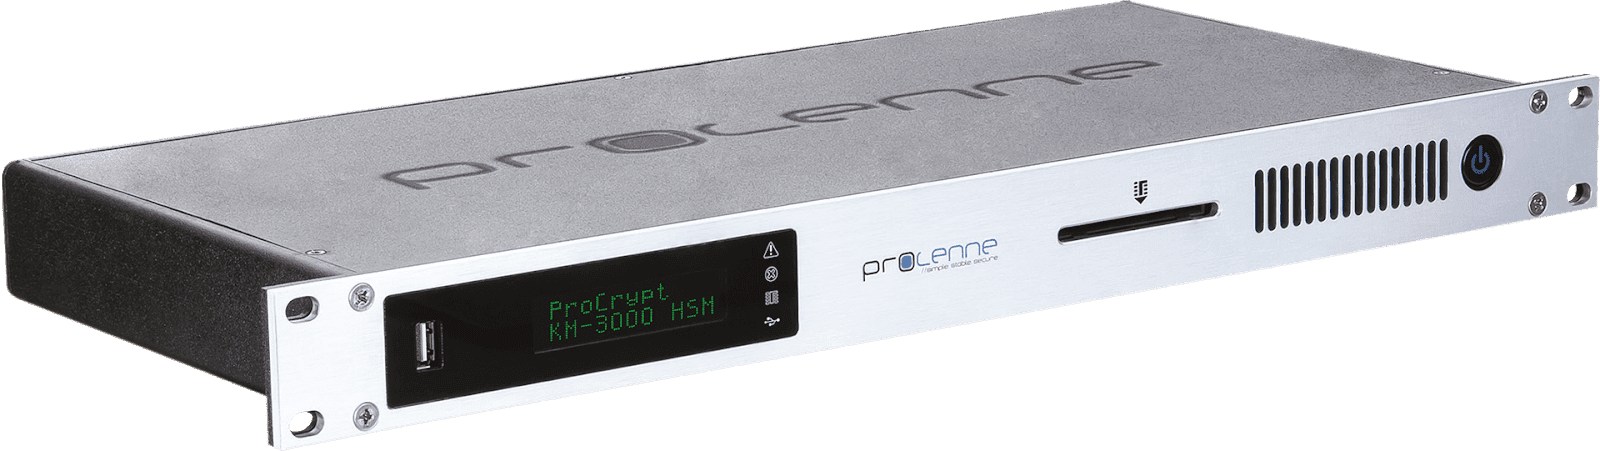
\includegraphics[]{2.hsm-example}}
    \end{center}
    \caption{Example of a General Purpose HSM, ProCrypt KM-3000 \cite{procrypthsm}.}
    \label{fig:hsm-example}
\end{figure}

Due to their crucial role in protecting infrastructures and applications, numerous standards, regulations, and certifications have been established to guarantee that general purpose Hardware Security Modules appropriately safeguard sensitive data and validate the effectiveness of the hardware performing cryptographic operations. Two internationally recognized standards are FIPS 140 \cite{fips140} and Common Criteria \cite{commoncriteria}. The former, Federal Information Processing Standard (FIPS), currently in the third version known as 140-3, is recognized around the world in both the public and private sectors, having four different levels of compliance \cite{fipslevels}, being the Level 3 the most common certification among the HSMs, while in the latter the majority of HSMs are certified at EAL4+, whereas the maximum EAL (Evaluation Assurance Level) is EAL7 \cite{commoncriteriacert}. In financial payment applications, the security of an HSM is frequently verified by comparing it with the standards established by the PCI SSC \cite{pcissc}.

The criteria used by FIPS to classify the effectiveness of the hardware performing cryptographic operations from Level 1 to Level 4 are the following: 
\begin{itemize}
    \item \textbf{Level 1:} The lowest level of security requires production-grade equipment and externally tested algorithms. There are no specific physical security requirements, and attackers can easily access and modify the module.
    \item \textbf{Level 2:} It adds requirements for physical tamper-evidence (the module must have a means of showing evidence of tampering, such as seals or locks) and a role-based authentication mechanism to control access to its services and functions. The module must perform additional self-tests and error handling.
    \item \textbf{Level 3:} A higher level of security than Level 2 that adds requirements for physical tamper-resistance (must have a strong enclosure that resists physical penetration and environmental attacks) and identity-based authentication (a mechanism that verifies the identity of the user or operator). The module must perform more rigorous self-tests and zeroize all sensitive data upon detection of tampering or abnormal conditions. There must also be a physical or logical separation between the interfaces by which critical security parameters enter and leave the module, and private keys can only be imported or exported in their encrypted form.
    \item \textbf{Level 4:} The highest level of security adds requirements for environmental failure protection, fault injection protection, and multi-factor authentication. The module must have a robust enclosure that provides a complete envelope of protection and detects and responds to any unauthorized attempts to gain access (tamper-active); must also protect against fault injection attacks that aim to bypass security mechanisms or induce errors; and implement a multi-factor authentication mechanism that requires the user or operator to present two or more independent factors of authentication, such as something they know, something they have, or something they are.
\end{itemize}

To summarize, the benefits of using Hardware Security Modules include:
\begin{itemize}
    \item compliance with security standards and regulations;
    \item high levels of trust and authentication;
    \item tamper-resistant, tamper-evident, and tamper-active systems to provide extremely secure physical systems;
    \item offering high levels of security for cryptographic keys and sensitive data;
    \item automated cryptographic key life cycle tasks that are fast and efficient, such as random generation, rotation, and protection of keys;
    \item keeping cryptographic keys in one location as opposed to multiple, unknown, and unprotected places;
    \item outstanding performance since it is designed and optimized for a specific and reduced number of tasks. 
\end{itemize}

\subsection{Virtual HSMs} \label{subsec:virtual-hsms}
Virtual Hardware Security Modules are a recent approach to overcome the high costs of these dedicated physical devices and their infrastructure \cite{hsmeconomics}. This alternative has the same responsibilities as the physical devices, including all its benefits, except outstanding performance since HSMs are specialized pieces of hardware and a virtual implementation would need to use other techniques to achieve the same security level we find in common HSMs, penalizing performance, resulting in a trade-off between performance, security, and expenses. These techniques can range from using Trusted Execution Environments (TEEs), such as Intel SGX \cite{intelsgx}, to employing a distributed system and using threshold cryptography to perform the cryptographic operations. Using this last strategy, instead of storing the cryptographic keys in a single location and device, these would be distributed among several servers, each storing a different portion of the original key, resulting in an adversary needing to compromise a determined number of servers to recover the key.


\section{Threshold Cryptography} \label{sec:threshold-cryptography}

Threshold cryptography corresponds to cryptographic algorithms where multiple parties are required to perform cryptographic operations, such as encryptions or signatures, employing a secure distributed protocol that allows the necessary secrets to be used collectively, revealing only the information about the output of the corresponding cryptographic operation. In contrast to depending solely on the security of a single trusted device, this alternative requires that a certain threshold of devices be compromised for an adversary to recover the secrets or violate security, which makes attacks more difficult to execute. Additionally, threshold cryptography is a distributed software-only implementation that aims to achieve at least the same level of security as the algorithms' centralized versions and, in some cases, provide even more security guarantees, namely when using secret sharing for safeguarding cryptographic keys instead of leaving them in a centralized place.

The growing enthusiasm for blockchains such as Bitcoin and Ethereum, the fact that these are moving towards signatures with simpler threshold versions, e.g., Schnorr~\cite{schnorrnotes} and BLS~\cite{blsdraft}, and the recent significant thefts involving the cryptocurrency side of these technologies \cite{cryptothefts2024} are examples that have contributed to reigniting the interest in this subject.  

Threshold cryptography can be divided into three main branches that will be covered next:\textit{ secret sharing}, \textit{threshold signatures}, and \textit{threshold symmetric encryption}.

\subsection{Secret Sharing} \label{subsec:secret-sharing}

A Secret Sharing (SS) scheme protects the confidentiality of the stored data/secret $s$ by splitting it into $n$ pieces, called shares ($s_1...s_n$). To later recover the secret, a portion of its shares must be combined; more specifically, $t + 1 \le n$ of these shares can recover $s$, and $t$ or fewer shares do not reveal any information about the secret. The number of available replicas is represented by $n$, while the maximum number of faulty replicas is symbolized by $t$.

This mechanism plays a vital role in creating a distributed virtual HSM and similar systems since it helps address the issue of securely storing private keys or secrets. Specifically, each replica stores only a share of the secret rather than all the data in clear or encrypted form. As a result, opposite to a single point of failure approach, if a replica is compromised, the adversary can only access the share of that replica, revealing nothing about the original secret.

There are two different major implementations of this scheme:
\begin{itemize}
    \item \textbf{Additive SS}: a simple algorithm where the secret $s$ is added to the remaining shares, corresponding to random values, $s + x_1 + ... + x_n$. Since all shares are required to reconstruct $s$, it can also be called non-threshold SS. This scheme is frequently used in the threshold ECDSA domain \cite{ecdsasurvey}, a threshold signature scheme covered in the next subsection.

    \item \textbf{Shamir SS}: the most popular implementation due to its flexibility in creating more complex schemes. In this scheme \cite{shamir}, the \textit{dealer}, responsible for the distribution of the shares, starts by building a random polynomial $P$ of degree $t$ such that $P(0) = s$ and generates each of the $n$ shares $s_1...s_n$ as points of $P$, $s_i = P(i)$. To recover the secret, the steps involved are: collecting $t + 1$ shares, interpolating the polynomial to recover $P$, and computing $P(0)$.
\end{itemize}

The original scheme, proposed by Shamir, had some limitations in the features it provided and has been improved to strengthen its security throughout the following years. A security aspect not initially available was integrity/verifiability, leaving the scheme vulnerable to active adversaries. This limitation can result in a malicious leader/dealer providing invalid shares or a malicious shareholder corrupting its share, leading the interpolation phase to output a different polynomial $P'$, in which $P'(0)$ will not result in the expected secret. \textit{Verifiable Secret Sharing} (VSS) solves this issue by extending the scheme with commitments. Basically, to each share $s_i$ is added an integrity proof, the commitment $c_i$, that allows shareholders and combiners to detect corrupted shares without revealing any information about the secret. A popular choice for VSS is Feldman's commitment scheme \cite{feldman}, based on exponentiations and the discrete logarithm problem.

As previously stated, secure storage of cryptographic data, such as secrets or private keys, is one of the most critical responsibilities of HSMs. This data type is typically used for extended periods, and over time, an adaptive adversary can corrupt some of the shares. To prevent these scenarios, the \textit{Proactive Secret Sharing} (PSS) scheme \cite{proactivess}, by regularly renewing shares, safeguards the confidentiality of data in long-lived systems against mobile adversaries who can ultimately compromise more than $t$ shareholders.

The aforementioned techniques are both combined in the \textit{Proactive Verifiable Secret Sharing} (PVSS) scheme \cite{pvss} to provide simultaneous share-renewal and verifiability.

Additionally, since these schemes are applied to distributed systems, which are always susceptible to changes in the available servers, alterations to the set of shareholders, including changing servers or even increase/reduce the group size and, consequently, change the threshold value, had to be supported without compromising the confidentiality of the secret. \textit{Dynamic Proactive Verifiable Secret Sharing} (DPVSS) \cite{mpss}, or just DPSS for short, is the term most commonly used to refer to the scheme that also includes this expertise. COBRA~\cite{cobra}, a substantial building block of our system, covered in Section \ref{sec:cobra}, uses it to accomplish confidentiality in BFT SMR systems.

\subsection{Threshold Signatures} \label{subsec:threshold-signatures}

A threshold signature scheme (TSS) enables a group of parties to collectively compute a signature without disclosing any information about their private key. In a $(t, n)$-threshold signature scheme, $n$ parties hold distinct key shares, where any subset of $t + 1 \le n$ distinct parties can issue a valid signature, but a subset of $t$ or fewer parties cannot.

The ultimate goal is to produce signatures in a threshold manner compatible with the existing centralized version of the same signature. In recent years, there has been renewed attention to this topic, primarily due to the development of blockchains. With a threshold signature scheme, the control of a cryptocurrency wallet, which is done through the corresponding private key, is distributed among $n$ servers such that $t + 1$ of them are required to produce a signature; hence, the funds will remain secure even if up to $t$ of these servers are compromised, which makes tampering a signature even more difficult.

With the early adoption of ECDSA in most blockchains, works on developing an efficient threshold version of the signature started to emerge \cite{gennaro18,lindell18,ecdsasurvey}. Nevertheless, ECDSA lacked an efficient way to compress and verify signatures; therefore, a new scheme to improve cryptocurrency scalability, efficiency, and privacy had to be employed. 

Nowadays, the most known and recognized blockchains are converging to a standard of signatures with smaller keys, non-interactive, and linearity schemes, as we can observe by Bitcoin and Ethereum, which began by using ECDSA and recently both received an upgrade where Schnorr and BLS signatures were incorporated, respectively.

Schnorr signatures \cite{schnorrnotes} are provably secure with standard cryptographic assumptions (discrete log), \textit{non-malleable} (a third party cannot alter a valid signature to create another valid one for the same key and message), and provide \textit{linearity}, which allows multiple parties to collaborate in producing a single signature valid for all public keys and enables signers in a multi-signature transaction to combine their public keys into a single aggregated key (key aggregation). Aggregating public keys into a single aggregated signature indistinguishable from a normal one reduces the block load. It also increases privacy since the list and the number of participants will be hidden \cite{schnorradvantages}. In contrast, multi-signature (multi-sig) approaches require each participant to produce an individual signature, which will be individually verified and recorded on-chain. This exposes the number of participants and their public keys, resulting in reduced privacy and an increase in on-chain data. 

BLS signatures \cite{blsdraft} rely on pairing-based cryptography and operate on unique curves, specifically pairing-friendly ones. This signature presents the same advantages as Schnorr, namely, enabling key and signature aggregation. However, the significant downside of BLS signatures is that verification is more inefficient and far more expensive than Schnorr, mainly due to the bilinear-pairing operations \cite{blsbetterthanschnorr}. Nonetheless, the ability to verify many signatures in batches overcomes this issue and can be very attractive for specific applications, particularly blockchains and cryptocurrency systems. 

Schnorr and BLS signatures, due to their linearity scheme, offer several advantages over ECDSA in terms of computational efficiency, storage, and privacy, as well as their simplicity in implementing them in a threshold manner. In contrast to the most recognized and efficient threshold ECDSA implementations, which require 13 communication rounds to complete the signing protocol \cite{lindell18,gennaro18}, or 11 rounds in a recent improvement \cite{gennaro20}, the threshold Schnorr and BLS versions require only two communication rounds to issue their signature.

A well-known implementation of threshold Schnorr signatures is FROST \cite{frost}; its specification was published in a draft standard \cite{frostdraft} and consists of a flexible, round-optimized scheme that minimizes the network overhead of producing Schnorr signatures. This scheme has also been the target of several improvements, both in terms of security and protocol efficiency \cite{frost3,frost3plus}.

Threshold BLS signatures are based on a straightforward combination of secret sharing and group operations and are specified in the IETF BLS signature draft standard \cite{blsdraft}. Tomescu et al. \cite{blsimproved} recently showed that an improvement to the efficiency and performance of the signatures aggregations could be made and proposed an adaptation of well-known fast polynomial interpolation algorithms to accomplish the computations in $O(t*log^2t)$ time, instead of the previous $O(t^2)$.

\subsection{Threshold Symmetric Encryption} \label{subsec:threshold-encryption}

A threshold symmetric encryption (TSE) scheme is a cryptographic operation that secures data by encrypting it in a distributed way, involving multiple participants. In this type of scheme, a predetermined number of participants (the "threshold") must collaborate to recover the original data, either by reconstructing the decryption key or performing a specific algorithm. Unlike traditional symmetric encryption, where a single key is used for both encryption and decryption, TSE ensures that no single entity holds the entire key, preventing unauthorized access even if one party's share is compromised. This approach is particularly useful for secure distributed systems that aim to ensure both confidentiality and resilience against attacks.

Multiple threshold cryptography schemes have been developed based on public-key cryptography, whereas symmetric-key schemes have not received the same focus and attention, leaving important security concerns and efficiency challenges to be resolved. Desirable features like each participant providing auxiliary data that can be used to check its partial result are supported in some threshold asymmetric cryptography schemes; however, symmetric-key encryption schemes, such as AES, do not offer this property due to the different nature of symmetric ciphers' algebraic structures.

A simple but insecure way of implementing threshold symmetric encryption is using secret sharing on the key of the authenticated encryption scheme, such as AES-GCM \cite{aesgcm}, where the key shares are sent to multiple parties, and then one of them reconstructs it to perform the encryption or decryption operation. Nevertheless, reconstructing the key negates the benefits of splitting it in the first place. Another approach would be to apply the secret sharing scheme directly to the plaintext instead of the key. While this avoids key reconstruction, it significantly increases communication and storage costs. Likewise, using secure multi-party computation (MPC) could be a possibility since it would allow keys to remain split during the operations, but it would also have a significant performance cost due to the required multiple rounds of high bandwidth communication between the parties. Therefore, high performance and efficiency can only be achieved by creating a dedicated threshold authenticated encryption algorithm.

The most recognized and well-known proposal for a threshold symmetric encryption scheme is DiSE~\cite{dise}. It presents the first formal treatment for \textit{Distributed Symmetric-key Encryption} (DiSE), which presents new notions of correctness, privacy, and authenticity in the presence of malicious attackers. The proposal consists of a generic construction of \textit{threshold authenticated encryption} (TAE) based on any distributed pseudorandom function (DPRF).

A DPRF is a distributed and interactive analog of a standard PRF. It is the main building block of DiSE, allowing a threshold number of distributed parties to collectively evaluate a function without reconstructing the shared secret. Initially, it involves a setup where each party obtains their share from a secret and the public secret sharing parameters. The DiSE and, in consequence, the DPRF start their protocol after receiving a commitment of the message to be encrypted sent by the client (or also called \textit{encryptor} or \textit{evaluator}). This input is collectively evaluated during the DPRF by any $t$ parties where $t$ ($\le n$) is a threshold. At the end of the DPRF protocol, only one party, the \textit{encryptor}, learns the output, a partial result sent by multiple parties that allows the \textit{encryptor} to assemble the final ciphertext and complete the DiSE algorithm. 

The chosen DPRF algorithm should meet two main requirements: (i) \textit{consistency}: the evaluation should be independent of the participating set, (ii) \textit{pseudorandomness}: the evaluation's output should be pseudorandom to everyone but the evaluator even if an adversary corrupts all other $t - 1$ parties and behaves maliciously. In this malicious case, a stronger property must be applied, (iii) \textit{correctness}: after an evaluation involving up to $t - 1$ malicious corruptions, an honest evaluator either receives the correct output or can detect the malicious behavior. Naor et al. \cite{naor} proposed and developed two very efficient two-round instantiations of DPRF, one based only on symmetric-key cryptography and another based on the Decisional Diffie-Hellman (DDH) assumption \cite{ddh}, being both used to provide the first formal proof of security for these constructions under a strong pseudorandomness requirement in DiSE.

In DiSE, the primary responsibility of the DPRF is to generate a pseudorandom key $w$ to encrypt the message $m$. For an adversary not to be able to reuse $w$ to create more than one valid ciphertext, the input provided to the DPRF is the identity of party $j$ concatenated with the message $m$, ($j||m$). 
This way, by placing $j$ inside the DPRF, a malicious attacker can not obtain $w$ by replacing the input of the DPRF in a new encryption query and thereby can not recover any message encrypted by an honest encryptor. Although the protocol checks for each party if a message $(j, \ast)$ comes from party $j$, this strategy reveals $m$ to all other parties, failing to achieve message privacy and efficient communication cost. To overcome this issue, a commitment of $m$ is sent to the DPRF. The hiding and binding property of the commitment ensures that $m$ remains secret and that $w$ is bound to this particular message. Nevertheless, the attacker could still generate valid ciphertexts by keeping $m$, $j$, and $w$ the same and using new randomness to encrypt $m$. This is prevented by making the ciphertext deterministic given $m$ and $w$: $w$ serves as input to a pseudorandom number generator (PRNG) to produce a pseudorandom string serving as a \textit{"one-time pad"} that is used to encrypt $m$ through an exclusive-OR (XOR) operation. 

Using an analogy with threshold signatures and using Figure \ref{fig:dise-simple-algo} as reference, the DPRF, for each server, will produce a deterministic partial result $k_i$, which the corresponding client that made the request will have the responsibility of aggregating them into the final ciphertext $c$ using the combined partial results $k$, with the desired message $m$ that was never shared with any of the available servers, but only a commitment of it, $t$.

\begin{figure}[h]
    \begin{center}
        \resizebox{120mm}{!}{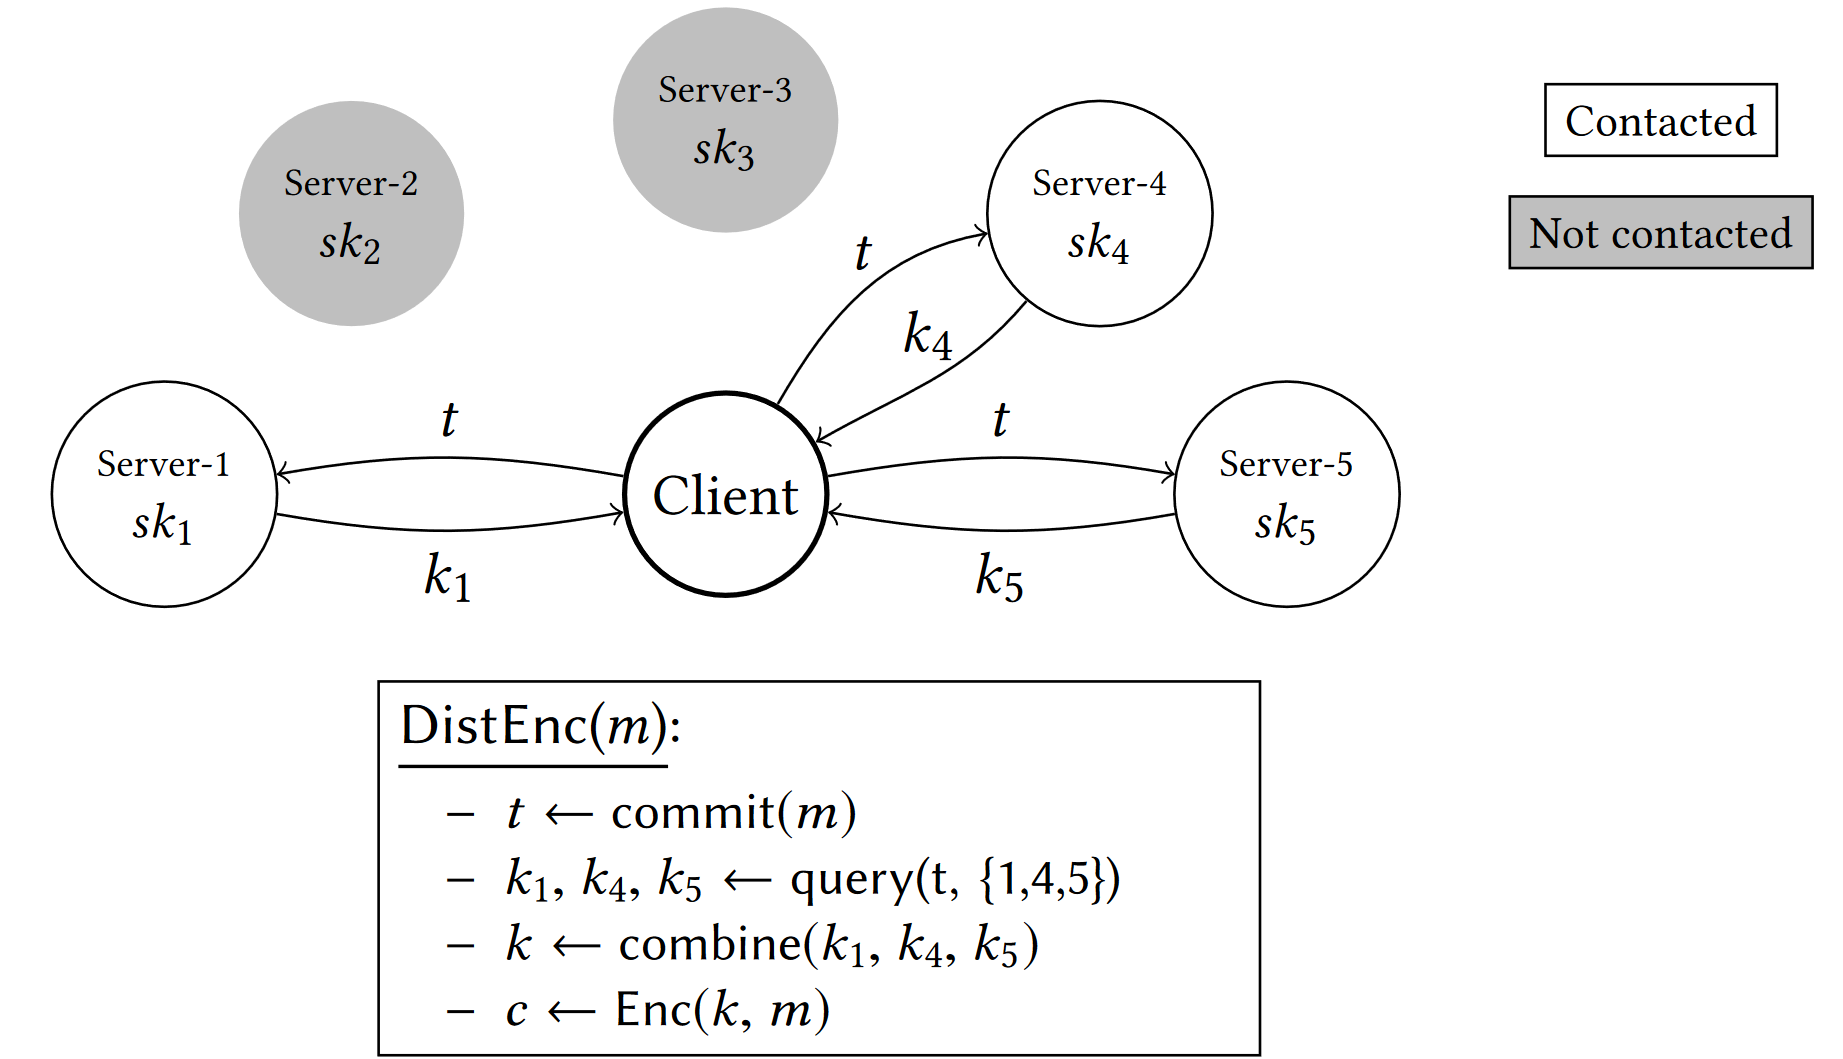
\includegraphics[]{2.dise-simple-algo}}
    \end{center}
    \caption{DiSE simplified protocol for $n=5$ and $t=3$ \cite{dise}.}
    \label{fig:dise-simple-algo}
\end{figure}

The DiSE protocol is composed of the following steps:
\begin{enumerate}
    \item Generate and distribute random symmetric keys to the $n$ servers;
    \item Upon receiving an \textbf{encryption} request from a client, any of the servers (say server $j$) can act as the \textit{initiator} (or \textit{encryptor}) to invite other ($t - 1$) servers to encrypt a message $m$ as follows:

    \begin{enumerate}
        \item Server $j$ first generates a long random number $\rho$ and calculates $\alpha = h(m \| \rho)$, where $h$ is a cryptographic hash function and $||$ denotes string concatenation;
        \item  Server $j$ chooses ($t - 1$) other active servers, sends ($j \| \alpha$) to them over secure channels, and asks them to return partial results $w_i$, so that $j$ can combine them into $w = \mathsf{DPRF}(j \| \alpha)$;
        \item Server $j$ assembles the final ciphertext $c = (c_1, j, \alpha)$, using a $\mathsf{PRNG}$, i.e., a pseudorandom number generator, where $c_1 = \mathsf{PRNG}(w) \oplus (m \| \rho)$.
    \end{enumerate}
    
    \item To perform the \textbf{decryption} operation, server $i$ agrees to act as the \textit{initiator}, or \textit{decryptor}, to decrypt a received ciphertext $c' = (c_1', j', \alpha')$, which may or may not be $c$ due to possible modification attacks.

    \begin{enumerate}
        \item Server $i$ chooses ($t - 1$) other active servers, which calculate $w' = \mathsf{DPRF}(j' \| \alpha')$, collectively;
        \item Server $i$, after receiving the necessary responses, computes $c' \oplus \mathsf{PRNG}(w')$ and parses the result into ($m' \| \rho'$);
        \item In the end, server $i$ checks the validity of the plaintext by verifying whether $\alpha' = h(m' \| \rho')$. If they do not match, ciphertext $c'$ has been tampered with and will be rejected.
    \end{enumerate}
\end{enumerate}

DiSE has been the subject of continued studies in the years that followed its publication, mainly due to the novelty and remarkable improvements made in the threshold symmetric-key encryption field, where the improvements were focused on the security guarantees and definitions, rather than changing the basis of the previously described protocol. 

\textit{Amortized Threshold Symmetric-key Encryption} (ATSE) \cite{amortizeddise} was one of the first works to provide improvements to the initial DiSE proposal. This work proposes a new primitive, formalized as \textit{flexible threshold key-derivation} (FTKD), to counter the necessity for interaction on each invocation of DiSE, which limits performance and incurs heavy computations and communication on the servers when encrypting large datasets.

\textit{Robust DiSE} \cite{robustdise}, on the other hand, intends to enhance the system's robustness by eliminating the honest-initiator assumption, introducing a rotating initiator role among active servers, and statistically detecting any attempt to use a compromised server repeatedly as the initiator, blocklisting the corresponding server.

\textit{ParaDiSE} \cite{paradise} is a recent proposal where Agrawal and other authors of the initial protocol revisit the problem of designing secure and efficient threshold authenticated encryption schemes. This work introduced new TAE security definitions to fix the issues found in the original DiSE proposal, namely definitions for capturing confidentiality, integrity, and preventing key reconstruction. In this new proposal, the authors departed from a more abstract description of TAE schemes and focused only on those operating in two communication rounds.

\section{State Machine Replication Systems} \label{sec:smr}

A state machine replication (SMR) system \cite{smr} is a strategy used in distributed computing to ensure that a group of replicas maintain the same state and perform the same operations in a deterministic and coordinated manner, i.e., in the same order, leading to consistent states across all replicas. This approach is crucial for building reliable fault tolerance and highly available distributed systems.

Distributed systems intended for real-world scenarios must use this approach combined with an effective and realistic fault model. The system we propose in this dissertation, a distributed and virtual HSM, must employ a Byzantine fault-tolerant SMR system since it is the classical method for implementing consistent and fault-tolerant services. This approach maintains the integrity and availability of a secure service, even if a fraction of the replicas fail in a Byzantine way. Instead of using a \textit{Crash Fault-Tolerant (CFT)} model, in which the fault would occur when a replica is faulty, that is, the system stops working or fails to respond, a \textit{Byzantine Fault-Tolerant (BFT)} model takes into account that a replica can behave arbitrarily or maliciously, sending incorrect or conflicting messages to other replicas in the system. This type of fault is more realistic and more challenging to detect and recover from because a faulty replica may try to deceive the others, causing the system to behave in unexpected ways, leading to inconsistencies and probably security vulnerabilities.

To avoid these issues, BFT SMR protocols are designed to tolerate these faults by ensuring that a correct replica can always progress despite the presence of faulty replicas. This is achieved through a consensus-based approach that requires a certain number of replicas to agree on the order of the commands to be executed. Another critical aspect of the underlying model of this type of system is communication \cite{commsmodel}.
In a \textit{synchronous communication model}, the messages are assumed to be delivered within a known and bounded time frame, simplifying the protocol design since it allows replicas to agree on the order of the commands even in the presence of Byzantine faults. However, this assumption is unrealistic in practice because network delays and failures are constantly occurring and can cause messages to be delayed or lost.
In contrast, in an \textit{asynchronous model}, the system assumes that messages can be arbitrarily delayed or lost, requiring more complex mechanisms to achieve consensus among replicas despite the presence of Byzantine faults.
Nevertheless, \textit{partially synchronous communication} \cite{partiallysynchronous} is the preferred model due to its realism and practicality. It accommodates real-world variability in message and processing delays by combining elements of synchronous and asynchronous models. This model ensures the eventual delivery of messages within certain bounds without requiring strict adherence to those bounds at all times, given that network and processes may behave asynchronously until some \textit{unknown} global stabilization time ($\mathsf{GST}$), which then become synchronous. This allows the system to handle temporary delays and network partitions while maintaining system performance and reliability. Algorithms designed for this model can optimize operations during synchronous periods and ensure safety and liveness during asynchronous periods. 

Examples of recognized works that produced protocols in the partially synchronous system model are Paxos \cite{paxos} and Raft \cite{raft}, protocols that solve consensus for CFT SMR systems, and also PBFT \cite{pbft} and BFT-SMaRt \cite{bftsmart}, which instead use the BFT model. PBFT was the first BFT protocol to achieve a performance similar to its CFT counterparts. BFT-SMaRt implements a library with a similar algorithm to PBFT that allows protocols that require a robust BFT SMR model to extend and use its functionalities, as is the example of COBRA, which is covered next.



\section{COBRA} \label{sec:cobra}

COBRA (COnfidential Byzantine ReplicAtion) \cite{cobra} implements confidentiality in practical BFT SMR systems through a new protocol stack for Dynamic Proactive Secret Sharing (DPSS). This framework, achieves high levels of security, consistency, robustness, fault-tolerance, integrity, and availability, and is an ideal candidate to be used underneath distributed systems that require these kinds of properties. COBRA did not directly develop some of these characteristics, but inherited from the library upon which it was built, BFT-SMaRt \cite{bftsmart}, a popular open-source BFT SMR library that provides essential BFT SMR features to the systems that extend it, including fault and asynchrony tolerance, crash recovery, and group reconfiguration.

Previous works that tackled the confidentiality issue in BFT SMR systems addressed the problem by integrating secret sharing with the consensus-based framework of BFT SMR. However, they did not provide several important capabilities for this type of system, such as replica recovery, group reconfiguration, and acceptable performance when handling a large number of secrets. Certain works, such as DepSpace \cite{depspace}, started using threshold cryptography, namely Verifiable Secret Sharing (VSS), to protect the confidentiality of stored data, providing a confidentiality layer for practical BFT SMR services. Nevertheless, those works did not consider adaptive mobile adversaries and adaptive sets of shareholders.

COBRA addressed these limitations with a novel approach for proactive verifiable secret sharing in dynamic groups of processes. The modular protocol stack consists of three main components: \textit{distributed polynomial generation}, \textit{share recovery}, and \textit{dynamic secret resharing}, represented in Figure \ref{fig:2.cobra-protocol-stack}. Together, these ensure that sensitive data is protected from adversaries and that the system can recover from failures without compromising confidentiality.

\begin{figure}[h]
    \begin{center}
        \resizebox{100mm}{!}{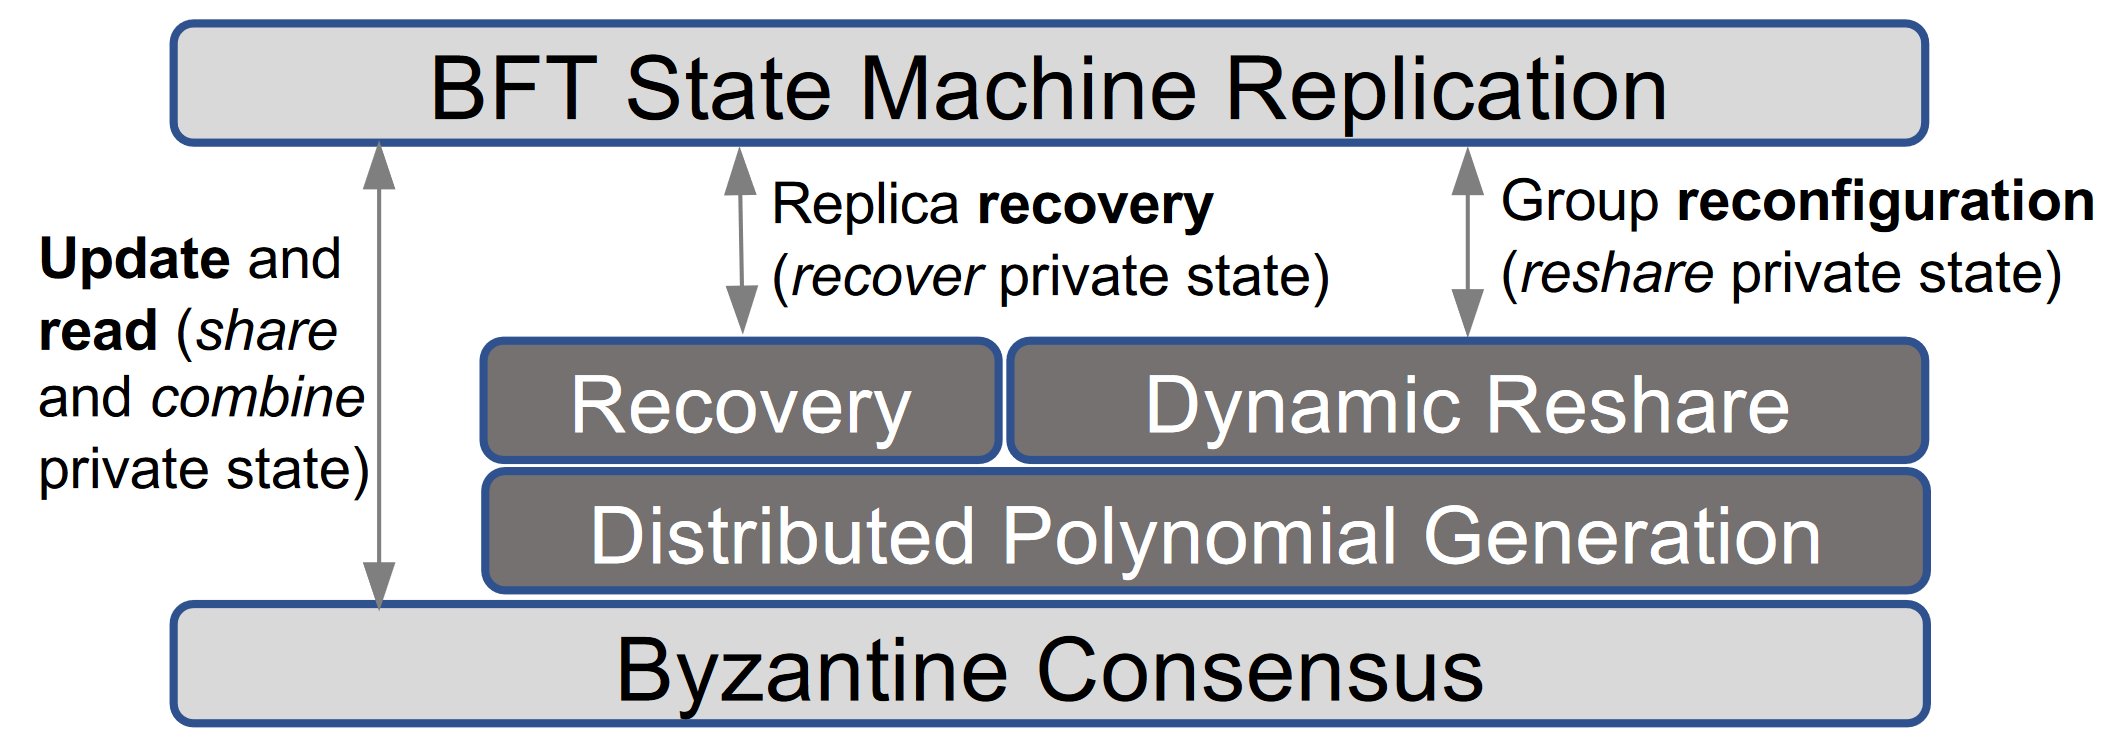
\includegraphics[]{2.cobra-protocol-stack}}
    \end{center}
    \caption{COBRA DPSS protocol stack represented by dark boxes \cite{cobra}.}
    \label{fig:2.cobra-protocol-stack}
\end{figure}

Furthermore, COBRA uses Byzantine consensus for \textit{distributed polynomial generation}. The distributed polynomial generation protocol allows replicas to jointly create new random and secret polynomials in a distributed way, with shares distributed to at least $t + 1$ correct servers, which is enough for their reconstruction. These polynomials serve as a basis for other protocols in the system stack: replica recovery, secret resharing, and group reconfiguration. To ensure the liveness of the consensus protocol employed, the authors assume a partially synchronous model \cite{partiallysynchronous} in which the network and processes may behave asynchronously until some \textit{unknown} global stabilization time ($\mathsf{GST}$), then become synchronous. To avoid some executions being adversary-influenced, the \textit{share recovery} requires $t + 1$ correct servers to rebuild the replica state, and the \textit{secret reshare} requires that all servers obtain valid renewed shares. This is done by the recovery protocol, which can identify and remove the processes that caused the generation of invalid shares during polynomial generation. This results in the correct servers re-executing the recovery protocol and ignoring messages from removed faulty servers, where eventually only correct servers participate.

Supporting replica recovery requires the re-generation of the replica's lost shares. When a server $r_i$ recovers from a failure, it needs (1) to obtain the common part \textit{C} of its state (which is replicated on other servers) using a state transfer protocol and (2) invoke the share recovery protocol for each stored data entry $D_j$, effectively reconstructing its private state. Regarding the state of the system, the \textit{Confidential SMR} service model contains a global system state \textit{S}, and locally each replica maintains two states, one common to all replicas \textit{C}, and one specific to each replica, containing the replica shares. The former is composed of $C = \{\langle\overline{D}_1, D^e_1, c_1\rangle, ..., \langle\overline{D}_m, D^e_m, c_m\rangle\}$: $\overline{D}_j$ is the non-sensitive data associated with the data entry (e.g., the key of a stored value, the metadata of a transaction in a blockchain), $D^e_j$ represents the data encrypted, and $c_j$ is the commitment for the shares of the encryption key. The private state of the replica contains the shares of the corresponding keys.

The COBRA paper presents an experimental evaluation of the system, considering up to 97 replicas and a state containing 100,000 stored secrets, showing that it is significantly faster than existing related work, for instance, resharing this number of secrets in a group of ten servers would require less than 12 minutes, which is, according to the authors, five times faster than Mobile Proactive Secret Sharing (MPSS) \cite{mpss}, a state-of-the-art protocol that uses a different technique to achieve DPSS.

Besides the critical features for practical BFT SMR systems inherited from BFT-SMaRt and the implementation of confidentiality in this type of system, allowing the secure storage of a large number of secrets, COBRA also supports replica recovery, secret resharing, share recovery, and group reconfigurations.

\section{Final Remarks} \label{sec:background-final-remarks}

This chapter started by identifying what hardware security modules are, specifically describing their main functionalities, responsibilities, and benefits, ending with a comparison between physical and virtual HSMs, highlighting their main differences. Next, we presented the main technologies that allow us to implement the system we propose in this dissertation, a virtual and distributed HSM that uses only software to develop and perform cryptographic operations. These technologies include threshold cryptography, namely, secret sharing, threshold signatures, and threshold symmetric encryption, followed by clarifying the concepts behind the systems we use underneath our implementation, that is, the BFT SMR system, which allows our project to be realistic and practical in the real world, and COBRA, a novel framework that added confidentiality to this type of system efficiently and securely.

\LIMPA

% Estado da arte

\chapter{Related Work} \label{chap:related-work}
This chapter discusses several related research directions with similar motivations and objectives that we also aim to achieve, although with different approaches. Firstly, we describe similar works related specifically to HSMs, and lastly, we present cryptocurrency wallets, what they consist of, and how they relate to our work.

\section{Virtual HSMs} \label{sec:virtual-hsms}
Some attempts have been made to virtualize HSMs, intending to reduce the high costs of these infrastructures while maintaining acceptable performance and achieving security guarantees as close as those present in the physical HSM devices.

\subsection{SoftHSM} \label{subsec:softhsm}

\textit{SoftHSM} \cite{softhsmgithub} is part of the OpenDNSSEC project \cite{softhsm} and was one of the first successful attempts to virtualize an HSM. Currently in the second version, specifically in 2.1.13, it is an open-source project still used today in testing environments, emulating an HSM for clients incapable of buying an expensive physical HSM. The software was implemented in the C++ language, and its features are accessible through a PKCS\#11 interface \cite{pkcs11spec}, which, among other functionalities, allows generating keys, issuing signatures, and performing encryption/decryption. However, since this system runs only locally on a single machine, it offers no real security guarantees and should only be used for testing purposes.


\subsection{pmHSM} \label{subsec:pmhsm}

\textit{Poor Man's Hardware Security Module} or \textit{pmHSM} \cite{pmhsm}, was also developed by DNSSEC and provides the same functionalities as SoftHSM; however, it offers better security guarantees with a different approach. To improve security and availability while maintaining the idea of virtualizing an HSM, the system was implemented as a distributed solution using threshold cryptography.

\begin{figure}[h]
    \begin{center}
        \resizebox{60mm}{!}{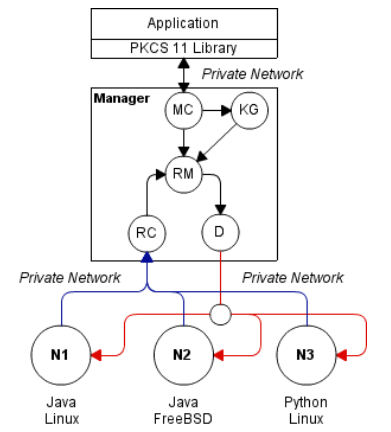
\includegraphics[]{3.pmhsm-arch}}
    \end{center}
    \caption{pmHSM architecture \cite{pmhsm}.}
    \label{fig:3.pmhsm-arch}
\end{figure}

The architecture of this virtual HSM is divided into three main layers, depicted in Figure \ref{fig:3.pmhsm-arch}: \textit{(i)} the \textit{application} that calls the functions of the PKCS\#11 API and translates them into messages to be sent to the next layer; (ii) the \textit{manager} that is responsible for receiving the requests from the application (e.g., signature, encryption, key generation), publishing them to the nodes and also waiting for their \textit{k} out-of \textit{n} responses, for instance, in case of a signing request, the nodes would send back to the manager a signature share; (iii) the \textit{shareholder} nodes correspond to the different replicas that communicate with the manager (in a \textit{publisher-subscribe} fashion), which receive the necessary information to complete the corresponding request (e.g., a document to sign in a signing request). 

In addition to the communications being transmitted synchronously between the servers, the main drawback of this work is that it is not a fully distributed solution. The manager acts as a trusted entity, sending and receiving sensitive cryptographic information, making it a single point of failure since the system depends on its honesty and availability. If an adversary manages to corrupt it, they can control everything and tamper with the messages as they see fit. Two protocols that would be directly affected by a Byzantine fault from the manager are: the key generation protocol, since the manager is responsible for generating the key and consequently possesses the full key and all its shares, given that it also has to create the corresponding shares using Shamir's secret sharing and also distribute them through the nodes; and the threshold signature scheme, considering that the private keys can be controlled by an adversary as well as all the signature shares that are received from the nodes.

Another weakness corresponds to the signature scheme employed, namely the threshold RSA signature scheme proposed by Victor Shoup \cite{practicalthresholdsignatures}, which is not as efficient as other recent protocols, not only due to the algorithm itself but also due to the need of bigger keys to achieve the same security level that other algorithms can achieve with smaller keys, as its the case of Schnorr and BLS, discussed in Section \ref{subsec:threshold-signatures}.

\subsection{Hardware-backed Virtual HSM} \label{subsec:rosahsm}

\textit{VirtualHSM} \cite{rosahsmthesis} corresponds to a project that developed a virtualized HSM supported by modern attestation-based trusted hardware in commodity CPUs to ensure privacy and reliability. The primary focus of this work was to develop a virtual HSM that could offer security guarantees similar to physical HSMs and achieve high availability through techniques like cloud-of-clouds replication on nodes equipped with trusted hardware. The proposed solution involves creating a virtualized and distributed HSM on the cloud, specifically utilizing Intel Software Guard Extension (SGX) \cite{intelsgx} enabled nodes for private key management, preserving the virtual HSM state, even if the node shuts down, by using an encrypted persistent data storage outside of the enclave, i.e., physical memory regions isolated from the rest of the system, including the operating system and hypervisor, where code can run with confidentiality and integrity guarantees provided by the hardware, in this case, Intel SGX. 

The downsides of this project are that it still requires the usage of trusted hardware and, although the authors claim it to be a distributed solution, it is more of a replicated centralized solution. This is because the HSM operations are performed on a single machine and, consequently, the security of the system is dependent exclusively on that machine's safety, specifically, the secure channels and the Intel SGX, as illustrated in Figure \ref{fig:3.rosahsm}. After a pre-defined number of executions resulting in state changes on a specific HSM machine, a batch with these changes is submitted to the other replicas.

\begin{figure}[h]
    \begin{center}
        \resizebox{130mm}{!}{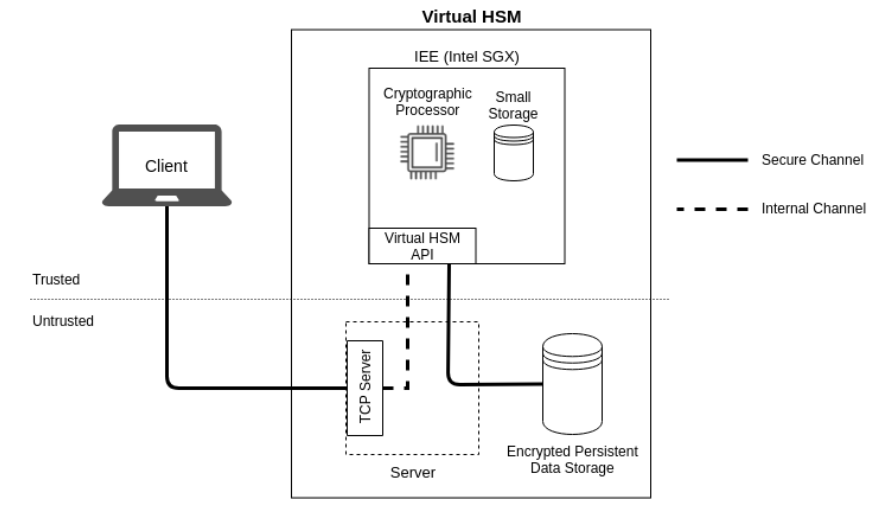
\includegraphics[]{3.rosahsm}}
    \end{center}
    \caption{VirtualHSM system architecture. The server acts as a proxy to securely connect the client with the Intel SGX, and this with the persistent storage \cite{rosahsmthesis}.}
    \label{fig:3.rosahsm}
\end{figure}


\subsection{Cloud HSMs} \label{subsec:cloudhsms}

\textit{Cloud HSM solutions} \cite{physicalvscloudhsm} enable users to quickly integrate high-performance cryptographic operations and secure key storage into their applications without the need to maintain on-premises appliances. Leading cloud providers offer fully managed HSM solutions that customers access via APIs and management platforms, the most popular of which are AWS CloudHSM, Azure Dedicated HSM, and Google Cloud HSM. These types of solutions offer no upfront hardware costs as the provider manages and operates the physical HSM infrastructure, provides a usage-based billing model where customers pay only for the time they use the HSM services, and delivers a seamless scaling through the provider as well as built-in high availability and redundancy. However, typically, these solutions work with physical devices and lead to customers having less visibility and control over the physical HSM devices owned by the provider. This can be a critical decision factor since the processed data is sensitive, and trusting a third party to store this type of information is always difficult. Moreover, even if there are no upfront costs to use this type of solution, but only an hourly fee for each HSM that is launched until it is terminated, the costs can also scale quickly. Using the AWS CloudHSM as an example, an HSM in Paris has an hourly price of \$2.18 per HSM, resulting, for a single HSM, in a monthly bill of \$1,591.40 \cite{awscloudhsmpricing}.


\section{Cryptocurrency Wallets} \label{sec:crypto-wallets}

Cryptocurrency wallets \cite{cryptowalletreview} provide customers the ability to send and receive digital currency through interaction with blockchains and can be referred to as software or hardware wallets:
\begin{itemize}
    \item \textbf{Software wallets:} Downloadable software programs that can be hot or cold, depending on whether it is connected to the Internet. Since nothing on the Internet is 100\% safe and money stored in a hot wallet is always vulnerable to theft, viruses, or loss due to software faults, these wallets are also more likely to be hacked. Moreover, these wallets can also operate in the cloud, and although convenient to access, it means that a third party controls the private and public keys stored in these wallets.
    \item \textbf{Hardware wallets:} Physical vaults that hold private keys on a hard drive specifically designed for that purpose. Although hardware wallets make transactions online, public and private keys are saved offline. 
\end{itemize}

These wallets, regardless of their type, should always provide a set of important features that complement their basic functionality of storing private keys and signing transactions, which include:
\begin{itemize}
    \item \textbf{Account creation:} Generate a pair of keys, a private key used to sign transactions, and a public key that acts as a public address, like an account number, used to interact with a blockchain, such as for accessing transactions associated with that address;
    \item \textbf{Key management:} Store and protect private keys. In a non-hosted wallet, the private keys are in the account owner's possession, while in a hosted wallet, a third party handles this task, and the account owner is unaware of the private keys. The organization handles the sending, receiving, and cryptocurrency storage on his behalf. Nonetheless, certain establishments do not keep personal keys; instead, they request them when needed;
    \item \textbf{View cryptocurrency balance and transactions:} This information is obtained from the blockchain using the user's public key;
    \item \textbf{User authorization:} Allow the user to access the wallet, which can be simply a PIN (Personal Identification Number) associated with the private key of the respective account;
    \item \textbf{User anonymity:} Send and receive funds anonymously by blockchain users. Anonymity is available on three levels: full, half, or less than half. A completely anonymous wallet does not request user information, unlike financial institutions that require users to register with all their personal information. If the mail ID is the only data needed to create or recover a password from a wallet, then the wallet is said to be half anonymous. Significantly less anonymous wallets collect a significant amount of data about their users;
    \item \textbf{Multicurrency support:} Enables users to use multiple cryptocurrencies inside of a single wallet concurrently;
    \item \textbf{Submit transactions:} Allows customers to move funds. The wallet signs the transaction with the private key, while the public key corresponds to the account of the receiver;
    \item \textbf{Wallet recovery:} If users forget their password or PIN, to prevent the coins from being lost forever, a widely used method is the seed phrase, a set of 12-24 random words used to recover access to the wallet.
\end{itemize}

Blockchains depend on cryptographic operations, and safeguarding private keys is imperative to protect the security of blockchain processes. Cryptocurrency wallets, as previously mentioned, are the connection to blockchains, and their main responsibilities are performing cryptographic operations and storing and protecting private keys, just like HSMs. The synergy between these technologies can contribute to improving the security of these systems; however, as stated before, physical HSMs are expensive devices, and since there are many cheaper centralized alternatives dedicated to cryptocurrency wallets, the investment might not compensate. This union is mentioned in some papers \cite{velinkhsmwallet,hsmbasedewalleteth}, where they use physical HSMs to secure private keys and to verify the user's identity through a PIN.

The theft of blockchain-based digital assets is a frequent reality \cite{cryptothefts2024}, and honest users should be protected from these events using different strategies. A secure cryptocurrency wallet should allow its user to divide their signing key among several devices and need all of them, or just a subset to complete a transaction, not enabling any single party to possess the signing key. Beyond splitting the key into multiple parts, the signature protocol being distributed will also allow each party to sign independently, using their portion of the key, where the final signature will be the combination of all the individual signatures. These types of systems can be achieved through threshold cryptography. 

Although there are publications regarding threshold wallets~\cite{goldfederwallets,bip32wallet,unstoppablewallet,proactivewallet}, their focus is primarily on threshold ECDSA signatures~\cite{gennaro18,damgard20}, which tend to have lower performance compared to non-interactive protocols due to the need for multiple communication rounds. Non-interactive signature schemes recently supported by blockchains, such as Schnorr and BLS, along with underlying wallet implementation features, such as, server recovery, server replacement, and secret resharing, are important characteristics of such distributed systems not addressed in these proposals. There are also proprietary solutions that implement threshold wallets; however, they do not disclose much information about the technologies and protocols used to achieve their results. Zengo \cite{zengowallet} and Blockdaemon Wallet \cite{blockdaemonwallet} are examples of organizations that developed solutions to protect digital assets by distributing operations using threshold cryptography, where both use Multi-Party Computation (MPC) to provide the security foundation for the corresponding services. The former uses an open-sourced MPC library maintained by the same company, while the latter uses a patented ``Advanced MPC protocol."



\section{Discussion} \label{sec:relatedwork-discussion}

In this chapter, we introduced the most recognized attempts to virtualize an HSM. SoftHSM implements a local solution for a virtual HSM, achieving a performance 15 to 20 times faster than the pmHSM, according to a comparison made by the authors. However, the first solution did not provide security guarantees, which was improved by the second version of the system by making it distributed, contributing to this difference in the obtained results. Additionally, the project developed by Miguel Rosa (VirtualHSM) achieved even better results mainly due to the fact that he uses dedicated hardware to perform cryptographic operations on a single machine, as in SoftHSM. The difference is that this work achieves necessary security guarantees, such as privacy, by using a trusted execution environment and availability by replicating the data among the servers.

Nevertheless, all the proposals present centralized or semi-distributed solutions, where some security properties are missing or are implemented differently than we intend to implement in our solution. As attempted by DNSSEC, the key to substantially lowering the costs of HSM infrastructures is not to try to beat the performance of the physical devices but to achieve the same security guarantees using other strategies. Therefore, we intend to implement a fully distributed solution, without any dependency on dedicated cryptographic hardware, that addresses the limitations of previous solutions, achieving the required security properties, including confidentiality, availability, and integrity, all in one system using threshold cryptography as well as a BFT SMR system, providing fault-tolerant features in the presence of Byzantine faults, which neither of the related works also offered. All these characteristics contribute to making a practical and realistic system in the real world.

Regarding cryptocurrency wallets, the objective is to develop secure implementations that can efficiently protect the digital assets of its users. The threshold versions of these wallets, although they can still be vulnerable to several attacks \cite{attackingthresholdwallets} if not correctly implemented, by using threshold cryptography to protect the keys, such as using secret sharing and also threshold signature schemes, the key is distributed in shares among different servers, requiring that an adversary compromises several of them to recover the private key.

\begin{figure}[h]
    \begin{center}
        \resizebox{120mm}{!}{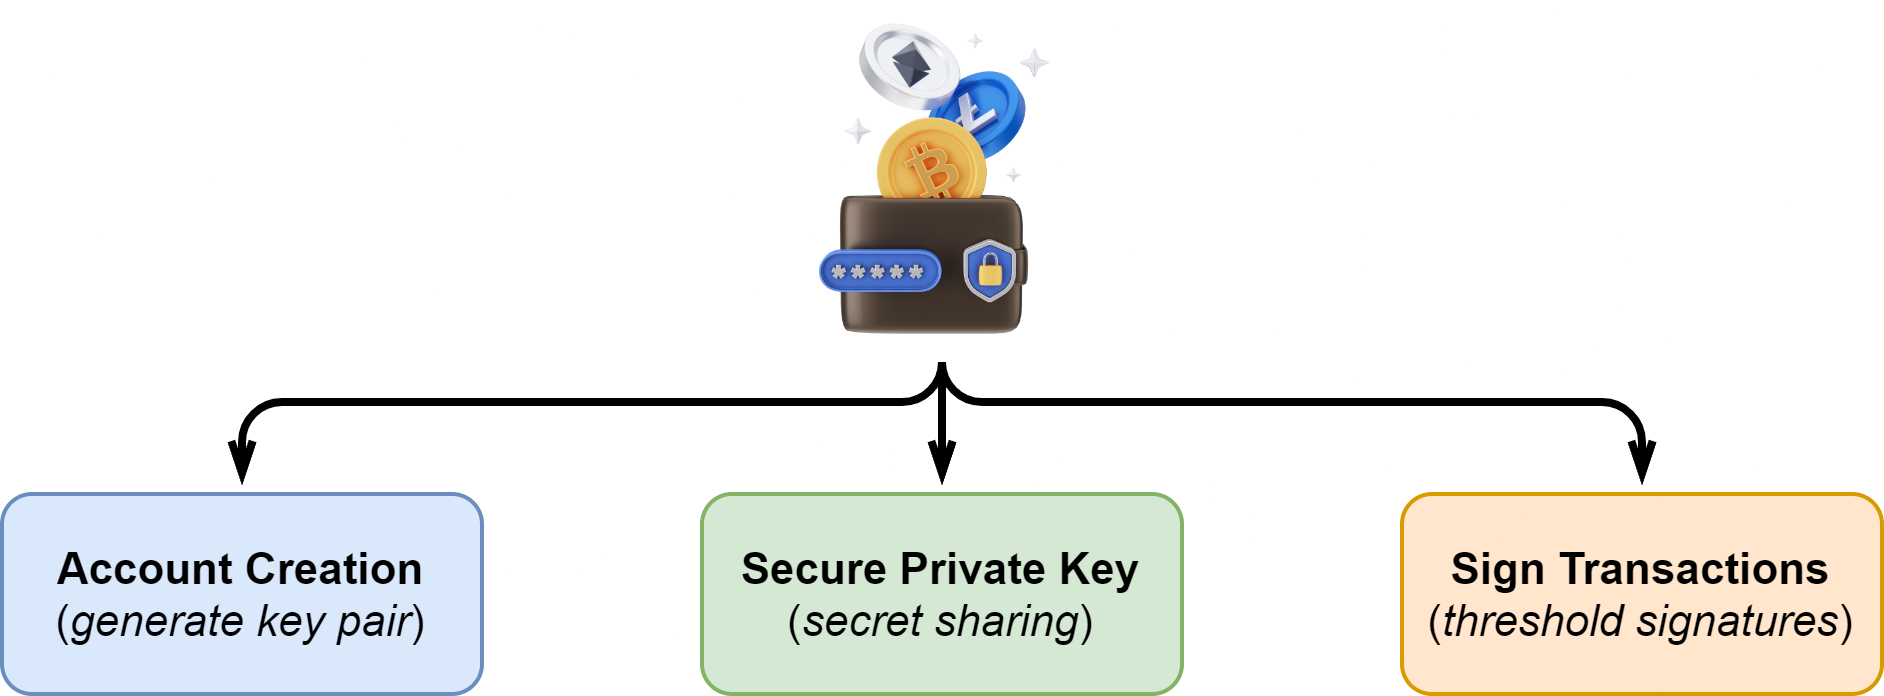
\includegraphics[]{3.cryptowalletfeatures}}
    \end{center}
    \caption{Cryptocurrency wallets main features supported by our system.}
    \label{fig:3.cryptowalletfeatures}
\end{figure}

Our open-sourced implementation, unlike proprietary solutions that require MPC protocols and public proposals that focus mostly on a single interactive signature scheme while neglecting important BFT SMR features for this type of system, represents a perfect use case for these wallets since it provides all the necessary threshold protocols to develop the most important functionalities, namely, account creation through generating keys in a fully distributed manner, safe storage of the private keys using secret sharing techniques, and transaction signing using only the shares of the key.

%\LIMPA

% Design
\chapter{System Design}  \label{chap:system-design}

This chapter details the system design of our Virtual and Distributed HSM, more specifically, the layers that compose our system and which contribute to its security in a distributed manner. It is followed by the system and adversary model, ending with an overview of the final architecture, where the roles and responsibilities of each component are described, as well as how they interact.

\section{Securing a Virtual HSM in a distributed way} \label{sec:securing-hsm}

A Virtual Hardware Security Module serves the same purpose as a physical HSM, but it exists only in the software environment and does not require any dedicated hardware to accomplish its normal cryptographic functionalities.

However, if we implement our system with only one server acting as a Virtual HSM, it would not be possible to achieve a similar level of security as a physical one since we would not have an isolated memory zone to protect sensitive data, such as keys, from the outside world; thus we would have a single point of failure that would certainly be an easy target for an attacker. Therefore, we had to implement our system in a distributed manner, and despite the difficulties and challenges this type of system causes, it allowed us to satisfy important properties, such as availability, integrity, and confidentiality.   

These properties are accomplished by combining several technologies and strategies in one system. Employing threshold cryptography protocols on top of a specific BFT SMR system allows us to develop a system with high availability, integrity, and confidentiality since if an adversary manages to compromise a replica, it would not reveal any information about the keys, nor would they be able to assemble the final result without compromising the other servers as well, which is very challenging to achieve. Moreover, the protocol and the system would keep functioning as expected due to the threshold strategy, where only a subset of the replicas are needed to conclude the operations, and even if an attacker tries to tamper with the system using counterfeit messages, the others can detect it by verifying the messages' integrity.

Furthermore, in order to implement a Virtual and Distributed HSM that aims to be practical and realistic, a BFT SMR system using a partially-synchronous communication model must be employed, since it is the classical approach for implementing consistent and fault-tolerant services. This approach maintains the integrity and availability of a secure service, even if a fraction of the replicas fail in a Byzantine way. As stated previously, our system was implemented on top of COBRA, which, besides the standard BFT SMR properties, also achieves data privacy, enabling us to take advantage of its features.


\section{System and Adversary Model} \label{sec:system-adv-model}

In terms of the system model, we consider a fully connected distributed system composed of a set of processes $\Pi$ divided into two non-overlapping subsets: a set of $n$ servers/replicas $\Sigma = \{s_1,s_2,..., s_n\}$, and an unbounded set of clients $\Gamma = \{c_1,c_2,...\}$. 
Clients access the system by requesting HSM operations, e.g., key generation, digital signature, and data encryption.

We assume a trusted setup in which each replica and client have a unique identifier that can be verified by every other process of $\Pi$ through standard means, e.g., a public key infrastructure. We suppress process IDs for readability when the processes involved are obvious. We further assume a partially synchronous model in which the network and processes may behave asynchronously until some \emph{unknown} global stabilization time ($\mathsf{GST}$), after which the system becomes synchronous, with \emph{known time bounds for computation and communication}. Finally, every pair of processes communicate through \emph{private and authenticated fair links}, i.e., messages can be lost and delayed, but not forever.

For the adversary model, we consider \textit{a probabilistic polynomial-time (PPT) adaptive adversary} that can control the network and may at any time decide to corrupt a fraction of the replicas in the current view. Replicas are allowed to deviate arbitrarily from the protocol, i.e., they are prone to Byzantine failures, and when corrupted, the adversary can learn the private state they store; however, if the failure threshold of each current view is respected, no confidential information can be obtained. More specifically, for a current view $\mathcal{V}$, the adversary can control simultaneously at most $\mathcal{V}.t = \lfloor\frac{\mathcal{V}.n - 1}{3} \rfloor$ replicas.

\section{Architecture Overview} \label{sec:arch-overview}

The high-level architecture of our system is illustrated in Figure \ref{fig:archvdhsm}, in which are represented two or more clients communicating with the system, specifically the servers that compose our virtual and distributed HSM, which exchange messages between themselves to resolve the received requests when it is needed. These requests are submitted by clients through the available Client API, which simplifies this process of requesting an operation by hiding all the necessary complexity underneath it. Ideally, clients would opt to use the PKCS\#11 API (also known as Cryptoki \cite{pkcs11spec}) to interact with the functionalities of a complete and standard HSM or the Crypto-Wallet API, which would be a simplified version of the Cryptoki API used by cryptocurrency wallets, that focuses basically on signatures and related features; however, we left these implementations for future work and implemented a simplified version that allows any client to interact with our system, and make use of the developed cryptographic operations. The specification of the Client API is described in the next subsection.


\begin{figure}[h]
    \begin{center}
        \resizebox{120mm}{!}{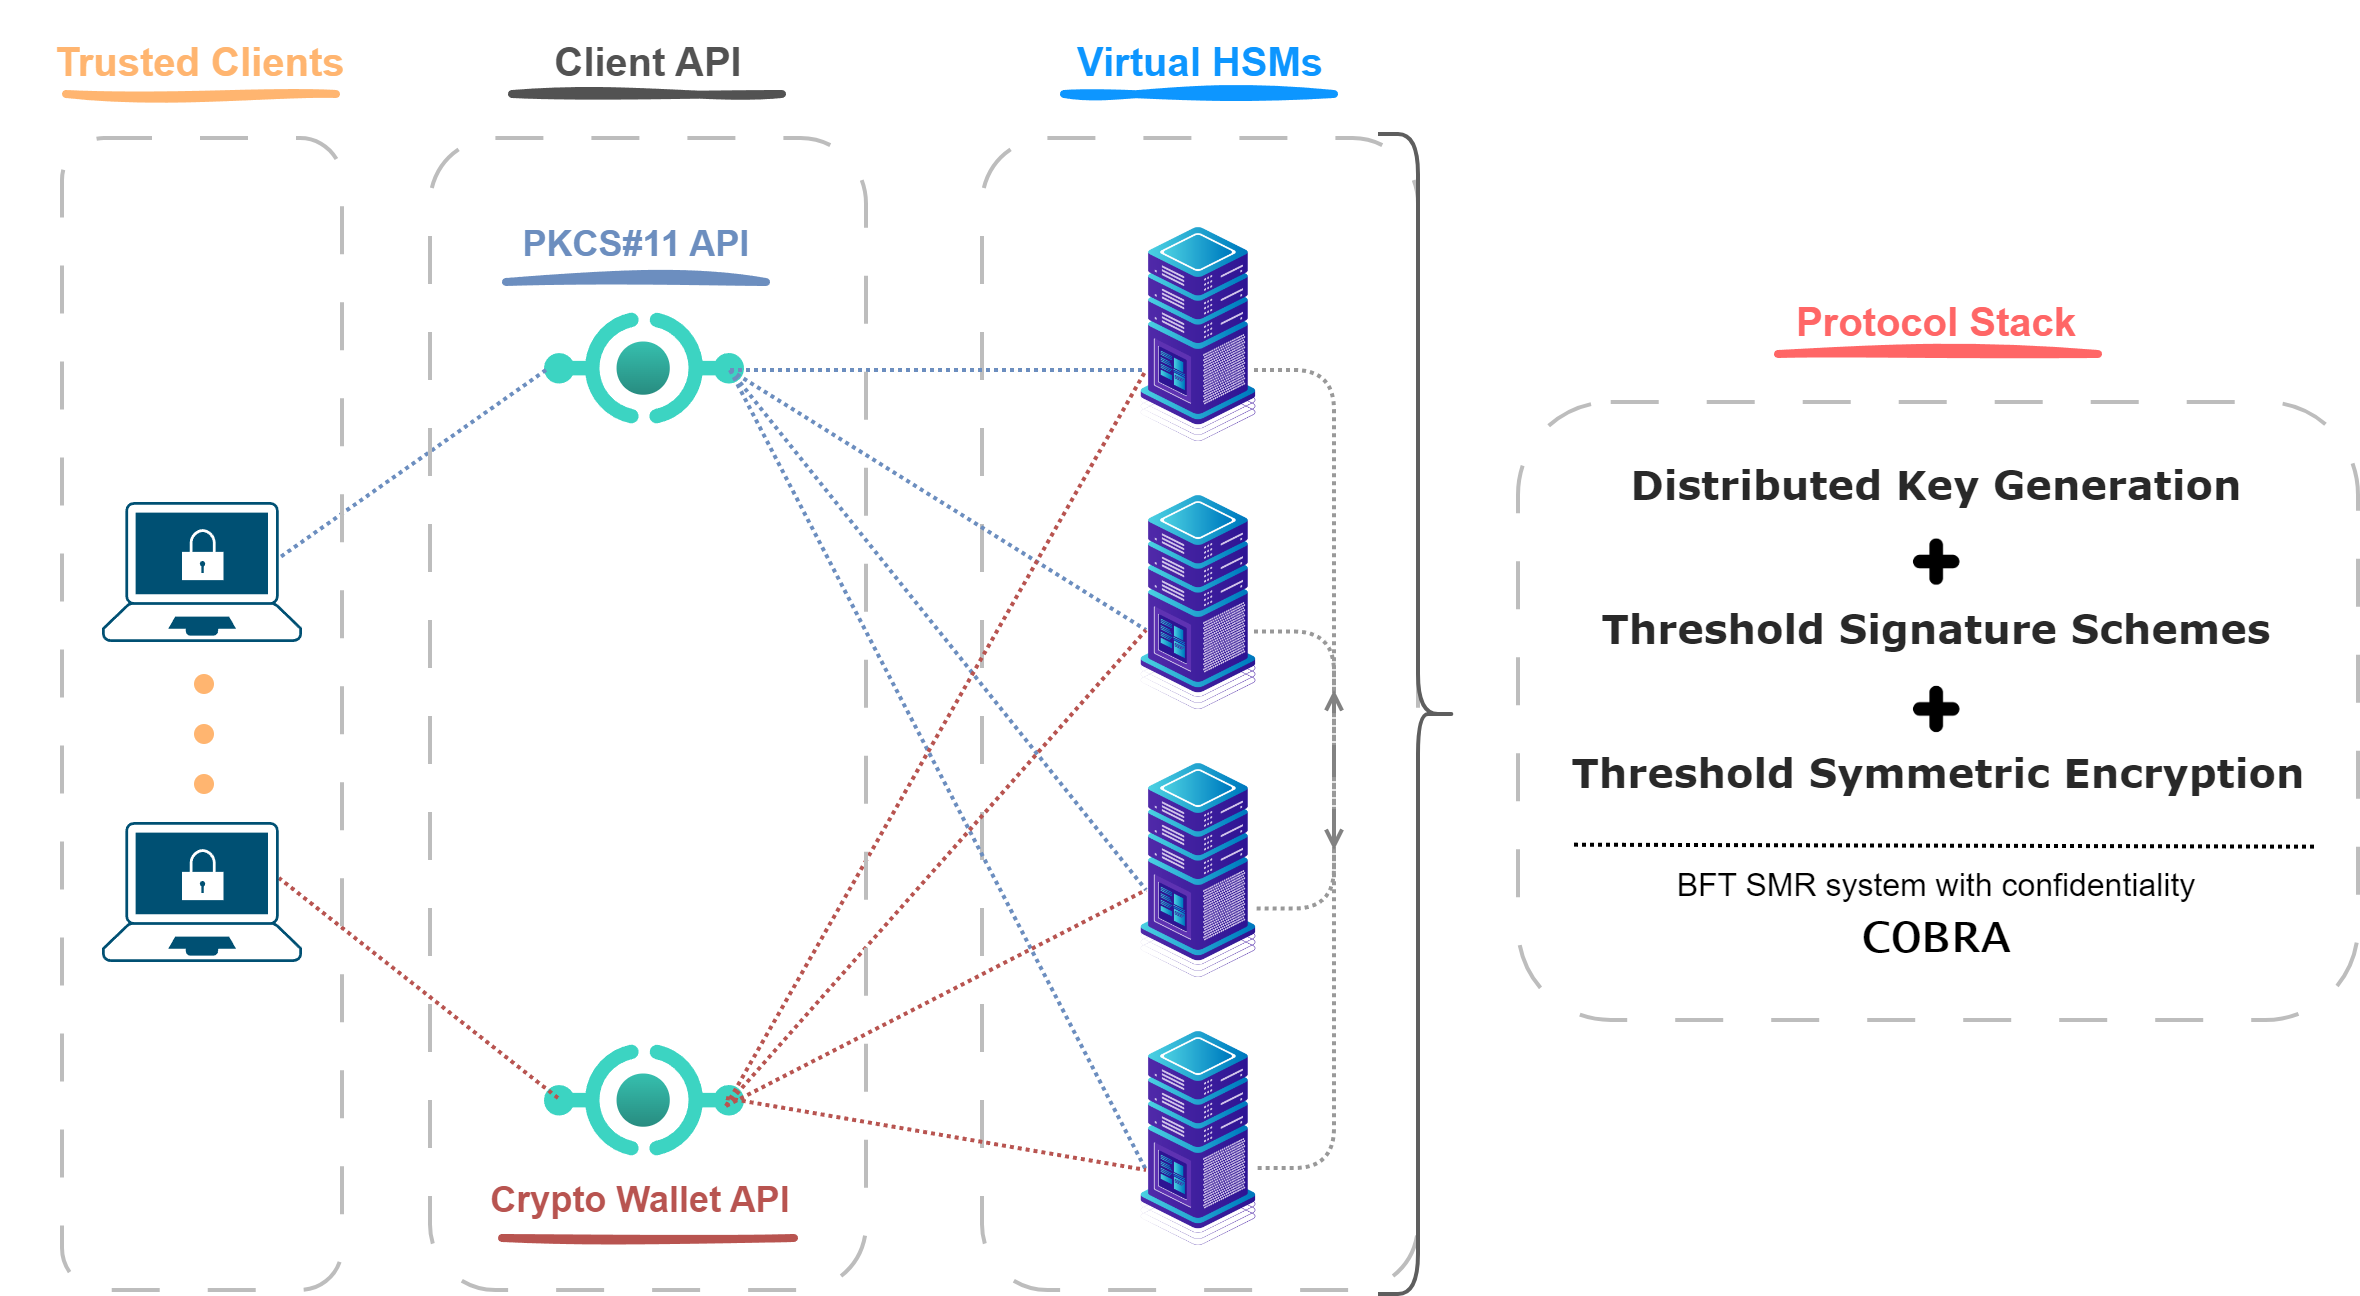
\includegraphics[]{4.system-arch}}
    \end{center}
    \caption{High-level architecture of our Virtual and Distributed HSM.}
    \label{fig:archvdhsm}
\end{figure}

Our system comprises the protocols that we have found to be the most efficient, secure, and practical since we were aiming for a system to be used in the real world. Our project's main algorithms correspond to a distributed key generation protocol, a threshold signature, and a threshold symmetric encryption protocol, as these are the distributed versions of the main features of a Hardware Security Module. Regarding the last two protocols, they follow a strategy where the replicas compute between themselves a partial result that each of them will send to the trusted client, which will be responsible for their aggregation into the final result, this being the signature or the final ciphertext. The protocols implemented in our Virtual and Distributed HSM are presented in the next chapter.

\subsection{Clients} \label{subsec:clients}
The clients are the system's entry point and must be trustworthy since they are responsible for initiating an operation and aggregating the partial results received into the final result. A compromised client would allow an attacker to manipulate the data sent to the servers, consequently enabling, for instance, the falsification of signatures or the decryption of any ciphertext previously issued by the same client. Hence, in our adversary model, we consider clients to be trusted.

To execute any of the available functionalities, a client needs to call the correspondent functions through the Client API, providing the required arguments depending on the feature being called.

The Client API covers and simplifies all the complexity of the implemented logic, making the available functionalities transparent to the final users. Specifically, it manages the encoding and decoding of messages sent and received from the servers, respectively, and the algorithms required for the partial results aggregation, which are exclusively produced by a specific set of the developed protocols, namely, signatures, encryptions, and decryptions.

The specifications of each of the functionalities available in the API are the following:
\begin{itemize}
    \item \texttt{generateKey(\textit{indexId}, \textit{keyScheme})$\longrightarrow$(success/$\perp$)}: Allows a client to submit a key generation request after providing the required arguments: \texttt{indexId}, i.e., a client unique index identifier that will be associated with the generated key that will act as a primary key in regular databases, allowing the client to select it or retrieve a previously generated \textit{public key}, in case of a asymmetric key pair, in the future; and \texttt{keyScheme}, a parameter that will allow generating the key for the correct finality, either selecting the proper elliptic curve for an asymmetric key generation (the currently available signature schemes are Schnorr and BLS schemes) or generating a symmetric key for the encryption operation. The result can either be a success message or $\perp$ if it was not possible to generate the requested key.
    
    \item \texttt{signData(\textit{indexId}, \textit{signatureScheme}, \textit{data})$\longrightarrow$(signature/$\perp$)}: Calling this function allows the client to issue a signature based on the provided arguments: \texttt{indexId}, the unique index identifier of the key to be used in the signature generation; \texttt{signatureScheme}, the scheme to be used when performing the signature, i.e., Schnorr or BLS, which must match with the one used in the selected key; and \texttt{data}, which corresponds to the data to be signed. In the end, the servers will respond with the issued signature or $\perp$, meaning that it was not possible to complete the signature protocol. Specifically, when successful, the client receives a pair containing the signature and the corresponding public key.

    \item \texttt{encryptData(\textit{indexId}, \textit{data})$\longrightarrow$(ciphertext/$\perp$)}: Function responsible for producing the encryption for the provided \texttt{data} using the key associated with the provided \texttt{indexId}. Returns the \textit{ciphertext} or $\perp$ if an error occurred and was not possible to finalize the encryption.

    \item \texttt{decryptData(\textit{indexId}, \textit{data})$\longrightarrow$(plaintext/$\perp$)}: Analogous to its encryption version, this function allows the decryption of the provided \texttt{data}, namely, a ciphertext previously generated by the encryption function using the key associated with the provided \texttt{indexId}. In the end, returns the initial \textit{plaintext} or $\perp$ in case it was not possible to conclude the decryption protocol.
\end{itemize}

The previously referred functions correspond to the most important ones since these implement the protocols studied in this project; however, the API still counts with some other utility functions:

\begin{itemize}
    \item \texttt{getPublicKey(\textit{indexId})$\longrightarrow$(\textit{publicKey}/$\perp$)}: Gets the \texttt{publicKey} associated with the private key that corresponds to the provided \texttt{indexId}. In case of an invalid or non-existent \texttt{indexId}, $\perp$ is returned.
    
    \item \texttt{validateSignature(\textit{signature}, \textit{publicKey}, \textit{data})$\longrightarrow$(\textit{Boolean})}: This function allows the verification of the validity of a produced \texttt{signature} using the correspondent \texttt{publicKey} and \texttt{data}, which is the data that was used to issue the signature in the first place. The function returns a \textit{Boolean}, specifically, \textit{true} if the signature was validated for the provided arguments or \textit{false} otherwise.

    \item \texttt{availableKeys()$\longrightarrow$(\textit{List<Keys>})}: Obtains from the servers the available keys the user requiring the operation has, returning a list of its keys, which specifically consists of the \textit{unique index identifiers}, the \textit{public keys}, and the \textit{signature schemes} used when generating each one of the stored keys.

    \item \texttt{commands()$\longrightarrow$(\textit{String})}: Client-side only operation that prints the available commands and how to use them properly.  
\end{itemize}


\subsection{Servers} \label{subsec:servers}
The servers are the most important component of our system since they implement the protocols that sustain the HSM service. Without them, we could not achieve the proposed objectives. 

Each server that composes our Virtual and Distributed HSM contains a stack of technologies that allow for the implementation of our distributed operations. Starting from the bottom layer, we have the library BFT-SMaRt \cite{bftsmart}, an implementation of a robust BFT SMR algorithm similar to PBFT \cite{pbft} that allows systems to extend and use its features, including state transfer for recovering a replica from a crash or slowness to the current state; reconfiguration of the set of replicas, allowing the addition or removal of replicas in runtime; and tolerance to faults, intrusions and asynchrony. The next layer is occupied by COBRA, a framework that implements confidentiality in BFT SMR systems using DPSS, particularly, extends BFT-SMaRt and adds on top of the previous features share recovery, secret resharing, and group reconfigurations without compromising the confidentiality of the stored secrets. The top layer, is where we implemented our cryptographic operations protocols. Our system takes advantage of all the features of the layers below, whether to ensure the security of secrets, making the system tolerant to intrusions, or simply using their communication manager to receive and respond to requests, all are extremely important to develop a practical and realistic system of this kind.

Basically, from a design point of view, upon receiving requests, the servers interpret them, execute the correspondent operation, and consequently, the matching protocol. Some operations require the servers to communicate with each other, being \textit{interactive}, while others are \textit{non-interactive}, meaning that the servers do not need to communicate between themselves to respond, each one only performs its own task and then send back the result to the client.

\begin{figure}[h]
    \begin{center}
        \resizebox{140mm}{!}{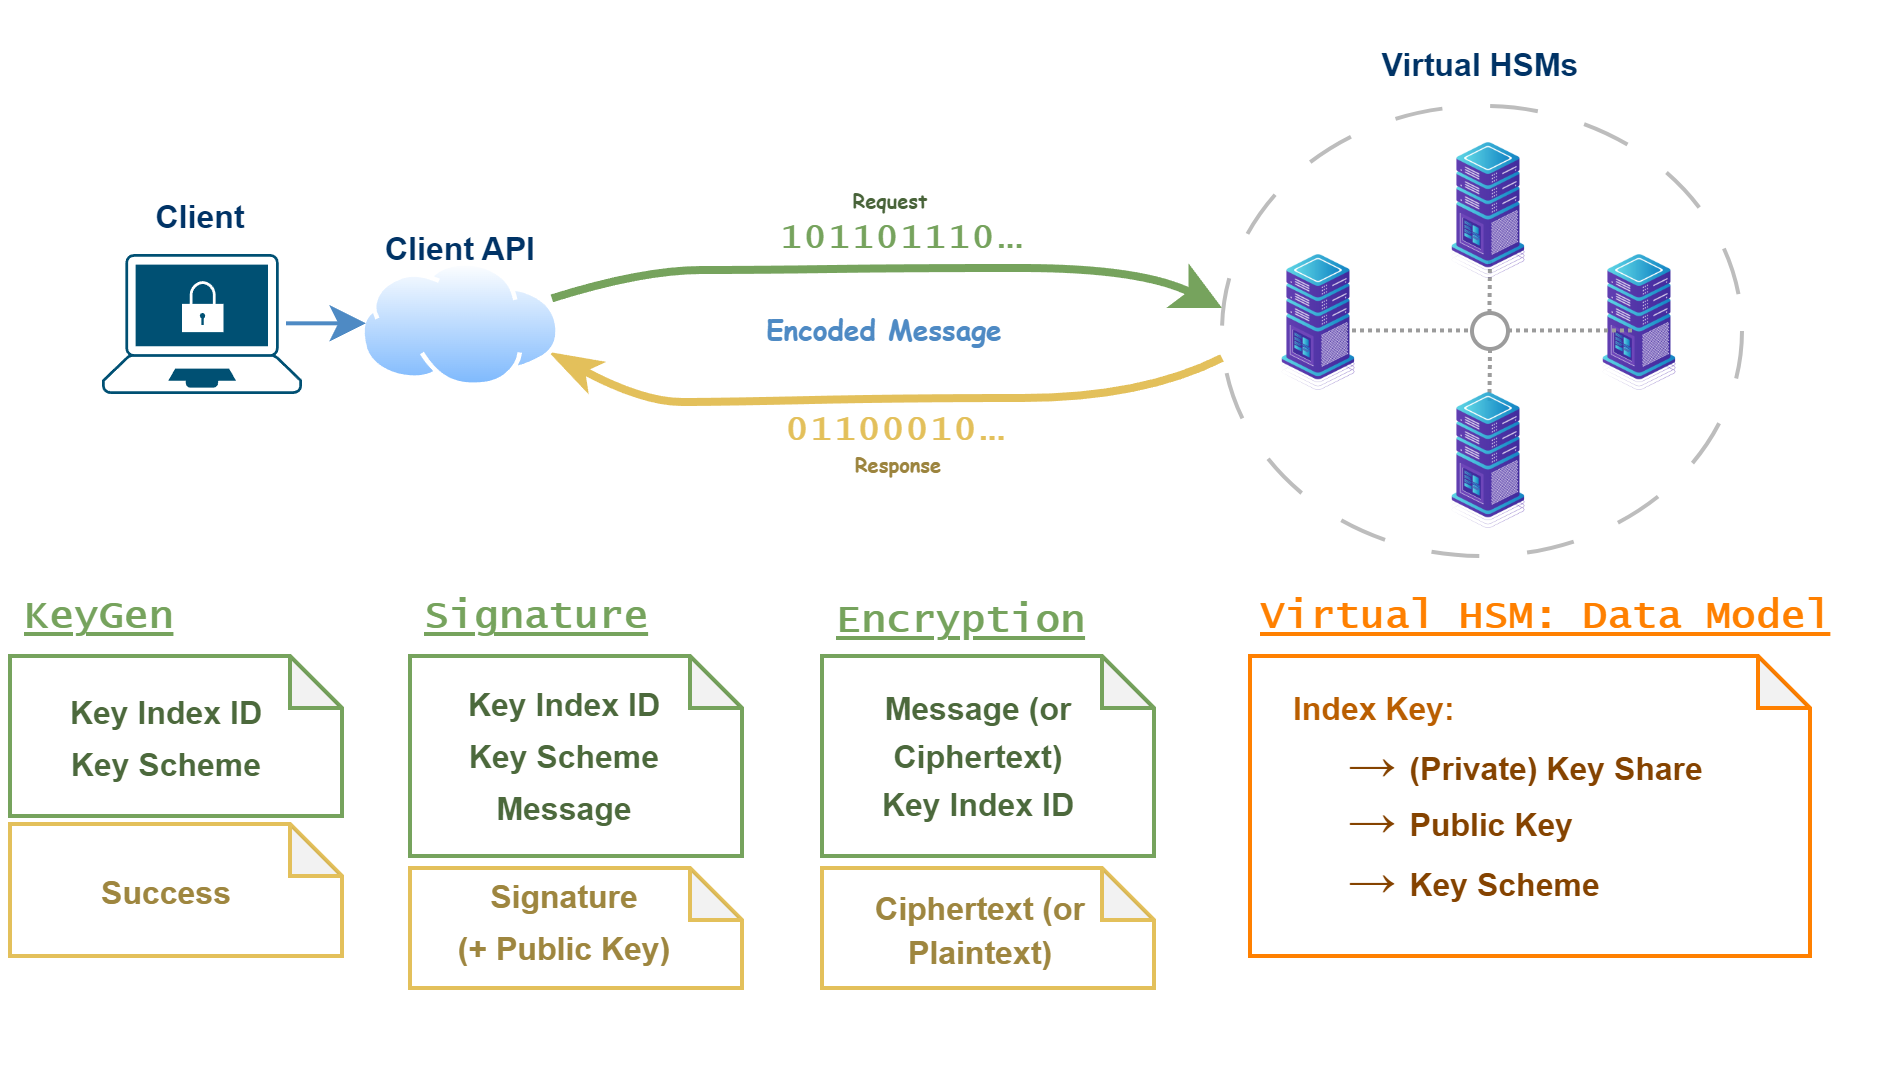
\includegraphics[]{4.data_model}}
    \end{center}
    \caption{Main operations and servers data model.}
    \label{fig:4.data_model}
\end{figure}

In addition to performing cryptographic operations, another main responsibility of our system, and HSMs in general, is safeguarding cryptographic keys. Each available server stores a share of the original private key, delivered by the Distributed Key Generation protocol to each one after the client requests the creation of a key. Specifically, each replica stores four different properties in its simple database (Figure \ref{fig:4.data_model}):
\begin{itemize}
    \item \textbf{Index Key}: A globally unique identifier, or primary key, associated with a generated key. This property allows clients to access their keys without conflicting with each other, because the identifier is composed of the \textit{client identifier} plus an \textbf{index identifier}, i.e., a client unique string submitted by the clients when requesting a key generation that will enable clients to distinguish between their stored keys;

    \item \textbf{Private Key Share}: Each replica stores a different portion of the generated private/secret key. The original key will never be reconstructed, and the shares will never leave their server;

    \item \textbf{Public Key}: To avoid spending time and resources to calculate a corresponding public key every time a client wants to retrieve one, we decided to store it alongside its corresponding private key;

    \item \textbf{Key Scheme}: The generated cryptographic keys are only compatible with a specific key scheme; therefore, we store that information to verify if the requested key scheme supports the provided key before starting the actual protocol. The available values that can be attributed to this property are \texttt{SCHNORR}, \texttt{BLS}, or \texttt{SYMMETRIC}.
\end{itemize}



\section{Final Remarks} \label{sec:design-final-remarks}

In this chapter, we discussed the design of our Virtual and Distributed HSM. Initially, we addressed the challenges of securing our system in a distributed manner, exposing how we achieve the most important properties that this type of system must have. All of those contribute to implementing a robust system that can prevail in a real-world environment. Next, we introduced the system and adversary model, presenting the assumptions made when implementing the project where the highlight goes to the clients, which we assume to be trustworthy. Therefore, the users are responsible for ensuring the security of their device, since it is there that the majority of the operations are completed. Afterward, we showed an overview of our system's architecture, followed by a description of the responsibilities of each major component, namely, clients, API, and servers. Specifically, we reveal the client's API end-users must follow when interacting with our system and the design of the data model implemented in the servers.  The next chapter discusses all the particularities of the system's cryptographic operations implementation.

% referir aqui que existem algumas funções que não requerem os servidores de comunicarem entre si, e dizer quais as operações e porquê 
%Regarding the servers' layers, there are some operations that do not require interaction between the servers due to their algorithm, namely, performing a BLS signature or an encryption/decryption. When these operations are received by the servers,  

%\LIMPA

% Implementation
\chapter{System Implementation} \label{chap:implementation}

This chapter describes the implementation aspects of our Virtual and Distributed HSM. Each section analyses a specific protocol, starting with the Distributed Key Generation, then the Threshold Signatures, and ending with the Threshold Symmetric Encryption. Each provides a more in-depth view of its features, implementation, and integration with COBRA.

\section{Distributed Key Generation} \label{sec:distributedkeygen}

A Distributed Key Generation (DKG) protocol is a fundamental building block of symmetric and asymmetric threshold cryptography. It solves the problems of single point of failure and key escrow, when there is a trusted authority that holds a secret, by using a complete distribution of shares of the secret among a set of servers, being the servers who will jointly agree on a secret, in contrast to the original secret sharing schemes \cite{shamir}, which required a leader to generate a secret and distribute its shares among participating parties.

The distributed polynomial generation protocol of COBRA \cite{cobra} served as the foundation for implementing our distributed key generation. This protocol does not require a designated leader to generate and distribute the shares of the secret. Instead, the protocol allows a group of servers to collectively create a random polynomial \textit{P} of degree \textit{t} with an encoded random point $(x, y)$ in a distributed manner. 

Each server in the group independently generates a random polynomial and distributes its shares to the other servers in the group. Subsequently, the servers run a Byzantine consensus algorithm to ensure that honest servers select the same set of $t + 1$ of these random polynomials. The selected polynomials are then summed, resulting in the shares of a polynomial \textit{P}. The protocol ensures that at least $t + 1$ correct servers obtain a valid share of the secret encoded in polynomial \textit{P}, and the other correct servers will detect invalid shares. This consensus process allows the servers to collectively agree on the shares of the polynomial \textit{P} without relying on a designated leader. The secret encoded in this random distributed polynomial can hence be used as a cryptographic key, remaining secret until a client decides to reconstruct it, which, in the case of our HSM, they never will as it is an operation that is not available. Nevertheless, since its shares are distributed throughout the servers, it can be used ``as is" for threshold signatures and encryption, i.e., without requiring additional client interaction.

To perform signatures with a specific algorithm, the required keys to issue the signature must follow a set of configurations, i.e., values that allow the construction of a distinct elliptic curve. The same signature algorithm can issue signatures using different elliptic curves, while others require a particular one. As we intended the system to be able to perform valid and compatible signatures for the Bitcoin and Ethereum blockchains, we would need to implement at least two different elliptic curve configurations. However, the previous protocol, and COBRA as a whole, were only compatible with the \texttt{secp256r1} elliptic curve, and the system was not prepared to be extended in this regard.

To work around this problem of being limited to a single elliptic curve, we had to guarantee that the functionalities that COBRA depends on would not be affected. With that in mind, we decided on the following solution:
\begin{itemize}
    \item When starting up the HSM replicas, for each desired elliptic curve, we initialize an instance of the \texttt{CobraConfidentialityScheme} class since this is the main class from where these configurations are called and obtained;
    
    \item The created instances are then registered in a map under the \texttt{DistributedPolynomial} class, which is the main class for generating the distributed polynomials. Each stored instance in the map is associated with the name of the elliptic curve it implements, acting as the entry key. We will be referring to it as \textit{confidentialitySchemeId};
    
    \item When a request is received, the \textit{confidentialitySchemeId} associated with the processed operation is propagated by the HSM servers to COBRA, so the correct scheme is used when performing the protocol;

    \item When executing the protocol, for all the servers to be in the same state and to avoid conflicts when receiving both different requests and signatures, we added the \textit{confidentialSchemeId} as a new field to the \texttt{PolynomialMessage} class, responsible for the messages that are changed between the servers during the distributed polynomial generation protocol. When decoding the received messages, it would enable each server to use the proper confidentiality scheme instance, obtainable from the initial map.
\end{itemize}%fazer uma figura com os passos que acontecem quando é recebido um pedido para gerar uma nova have

This way, the system will not be limited to only one or two elliptic curves but to an arbitrary number of different ones, requiring only the configuration of the desired curves in the \texttt{HsmServer} file, although these also need to be compatible with the available algorithms.

At the moment, besides the native one that was previously installed, \texttt{secp256r1}, the system supports two new elliptic curves, \texttt{secp256k1} and \texttt{BLS12-381}, enabling the creation of cryptographic keys compatible with the Bitcoin and Ethereum blockchains, respectively, since cryptocurrency wallets are a use case of our project. These two last curves allow for the generation of keys compatible with two different signature schemes, Schnorr and BLS, respectively, which will be covered in the next section. 

The DKG protocol enables the creation of a secret or a private key depending on the final purpose. Therefore, when generating a private key, the corresponding public key is created differently depending on the signature scheme. In the protocol implemented for the Schnorr signature, the public key corresponds to the commitment of the generated private key, while for the BLS scheme, we use a third-party library to create a compatible public key. Regarding symmetric keys, since our encryption algorithm is not a traditional protocol, it does not require a specific type of symmetric key, so for this case, we simply generate a secret key using the DKG protocol, which, in our case, will act as a symmetric key in a centralized encryption algorithm. 

\section{Threshold Signatures} \label{sec:thresholdsignatures}

With the help of a threshold signature scheme (TSS), multiple parties can jointly calculate a signature without sharing any details about the private key. Schnorr and BLS signatures were chosen to be implemented since they are non-interactive and present advantages related to simplicity and performance. They were recently implemented in the most known blockchains, Bitcoin and Ethereum, respectively, eventually leading to smaller blockchains following their steps.

To implement the Schnorr signature \cite{schnorrnotes} in a threshold manner we utilized a version of the protocol already implemented in the SIRE project \cite{siregithub}, which was inspired by the ROAST proposal \cite{frost3}, and for the BLS signature \cite{blsdraft} we used the RELIC library \cite{relicgithub} which already provides all the necessary functions to sign, combine, and verify the signatures and key pairs. Both schemes allow the aggregation of partial signatures into a final signature, and the BLS signatures enable the grouping of private/public keys into a single key pair. Therefore, each server starts by producing its share of the signature, i.e., a partial signature and public key, and then, the client is responsible for combining them into the final signature and public key.

As previously stated, the high-level algorithm of both signatures corresponds only to a two-round client-server communication. During the first, the client submits the request with the necessary information to issue the signature, specifically, a hash of the message to be signed, the index ID of the private key to be used, and the signature scheme. In the second round, the servers respond with a partial signature constructed using the private key share each of them possesses. After receiving the required number of partial results, the client verifies their integrity and combines them into the final signature.

Regarding the Schnorr signature scheme, the algorithm performed by each replica to generate the partial signature is very similar to the regular centralized version. After the replicas conclude the distributed key generation protocol, due to the need for a random value $k$, they start by computing a hash $H$ of the data to be signed $M$ with the public key of the generated value $r$, $e=H(M || r)$, where $||$ denotes concatenation. The partial signature is completed by computing $s_i=k_i + e \cdot sk_i$, where $sk_i$ corresponds to the private key share associated with the index ID provided by the client. When the partial signatures are received, the client verifies them using the commitments of both the private key and the random key value, which were sent with the partial results, and then combines them into the final signature using the Lagrange Interpolation with the valid partial signatures. Due to the need for a new random key value for every Schnorr signature to avoid a possible key leakage from reusing this nonce, the key generation and the Schnorr signature operations are the only ones that require the replicas to communicate among themselves since we need to invoke the DKG protocol again to generate this random value.

Concerning the BLS signature scheme, we use the RELIC library~\cite{relicgithub}, a modern research-oriented cryptographic toolkit emphasizing efficiency and flexibility implemented in the C language, to compute the signatures. An exciting feature of this scheme is that the signatures and public keys can act as final or partial values, depending on our objective. Just like in threshold Schnorr signatures, the only difference when calculating the signature to become threshold is that where the private key was used, we now replace it with the private key share instead, $s_i=H(M) \cdot sk_i$. We use this library to calculate the public key share (corresponding to the private key share stored by each replica), issue the signatures using the private key share, verify the signatures' validity, and perform the Lagrange Interpolation to build the final signature and public key.


\section{Threshold Symmetric Encryption} \label{sec:thresholdencryption}
% talvez fazer uma figurinha com o funcionamento do algoritmo, tipo o client envia um pedido, com o commit da data, e cada servidor envia a sua contribution para o client, este constroi o ciphertext, e mais tarde envia o commit de volta para o servidor para realizar a decryption, que corresponds aos mesmos passos da encryption.

To achieve a practical and efficient threshold symmetric encryption, we implemented the most distinguished proposal in this field, discussed in Section \ref{subsec:threshold-encryption}, named \textit{Distributed Symmetric-key Encryption} (DiSE) \cite{dise}. The idea of the protocol consists of a generic construction of threshold authenticated encryption based on any distributed pseudorandom function (DPRF), where each server produces a partial result that the client will then combine to produce the final ciphertext, or the original message when performing the decryption. 

A technical view of the implemented protocol is illustrated in Figure \ref{fig:5.3.dise-protocol}. To adapt this algorithm to our system, we utilize our DKG protocol to generate and distribute the secret key shares among the replicas, and as the authors did in their implementation, we use \texttt{SHA3-256} as a commitment scheme and the AES algorithm as the pseudorandom number generator. Specifically, as described in the API specification of the previous chapter, the clients will first generate a secret key using the DKG (which we consider to be our symmetric key), so later they can use the pre-generated secret key to perform an encryption or decryption by providing the \texttt{indexId} associated to the key during its creation.

\begin{figure}[h]
    \begin{center}
        \resizebox{80mm}{!}{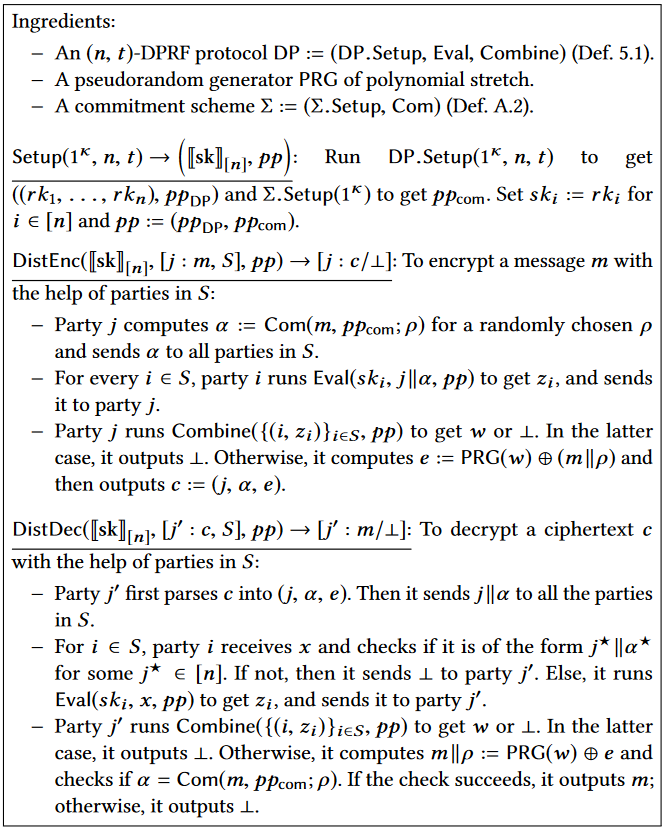
\includegraphics[]{5.3.dise-protocol}}
    \end{center}
    \caption{The implemented DiSE protocol \cite{dise}.}
    \label{fig:5.3.dise-protocol}
\end{figure}

The DPRF is the algorithm's most crucial component. Its responsibility is to generate partial results deterministically. Being deterministic is the key factor for making possible a later decryption of a ciphertext previously encrypted by this same protocol.

The applied DPRF was inspired by the algorithm depicted in Figure 6 of the DiSE paper~\cite{dise}, corresponding to a privately verifiable version, secure under the Decisional Diffie-Hellman assumption~\cite{ddh}, that requires only two communication rounds to conclude its protocol. It was adapted by Robin Vassantlal, author of COBRA, joining it to a previous version of a DPRF that he had implemented when developing his project, adjusting the protocol to support the usage of elliptic curves. Afterward, we extended this implementation to use the Distributed Key Generation described above in its setup phase, allowing each replica to agree on a polynomial and obtain their shares in a distributed manner. The final version of the DPRF algorithm contains the following steps:
\begin{itemize}
    \item \textbf{Init:} Performs the DKG protocol, distributing the secret key shares among the servers $(sk_1, ..., sk_n)$ and sets the constant parameters, i.e., the elliptic curve configuration, where $g$ corresponds to the curve generator which is the $(x, y)$ point in the curve, and $rho$, corresponding to the curve's prime order. In the end, each server's private and public parameters ($pp$) are obtained. The former contains the secret key share, which never leaves the corresponding server, and the latter holds the commitment of the key share ($com_{sk_i}$), being the only information sent to the client;

    \item \textbf{Contribute}$(sk_i, x, pp)$: Computes $w = g \cdot x$ and $h_i = w \cdot sk_i$. Picks $v_i \leftarrow \mathbb{Z}_\rho$ and sets $t_i = w \cdot v_i$. After calculating all these variables, computes the final hash $c_i = \mathcal{H}(h_i, w, com_{sk_i}, g, t_i)$ and $u_i = v_i - c_i \cdot sk_i$. Resulting in the output $z_i = (h_i, c_i, u_i)$, which corresponds to the partial result;

    \item \textbf{Evaluate}$({(i, z_i)}_{i \in S}, pp)$: If the number of received contributions $S$ is less than the required $t$, return $\perp$. Otherwise, parse $z_i$ as $((w, h_i), (c_i, u_i))$ for $i \in S$. Compute $t_i = w \cdot u_i + h_i \cdot c_i$ and check if $c_i = \mathcal{H}'(h_i, w, com_{sk_i}, g, t_i)$. If check fails for any $i \in S$, return $\perp$, else return $\sum_{i \in S}h_i \cdot \lambda_{0, i, S}$, where $\lambda_{0, i, S}$ correspond to the Lagrange coefficients.
\end{itemize}

A key characteristic of this algorithm is that the clients send to the servers only a commitment of the data they want to encrypt. This way, the size of the data will not influence the system's performance. The commit corresponds to the hash of the data to encrypt together with a random value, allowing the initial data to remain secret to the servers throughout the entire process.

In the end, the resulting ciphertext includes the identifier of the \textit{encryptor}, i.e., the client's identifier who aggregated the partial results into the final ciphertext, the committed data, and the actual encryption. Later, if not tampered with, these additional properties will allow the protocol to retrieve the corresponding initial message.

\section{Final Remarks} \label{sec:impl-final-remarks}

In this chapter, we detailed the implementation particularities of each main protocol. We demonstrated how these algorithms achieved the previously referred properties of confidentiality, integrity, and availability by explaining each in-depth. We started with the Distributed Key Generation protocol, where, besides providing details of the algorithm, we clarified how we resolved the problem of expanding the protocol to allow the usage of any elliptic curves. Then, we elaborated a simplified version of the algorithms employed for the threshold signatures, namely, Schnorr and BLS signature schemes. Finally, we introduced a more technical description of the threshold symmetric encryption protocol utilized, DiSE. Specifically, we defined the chosen DPRF protocol and noted all the changes to adapt it to our needs. 

%\LIMPA

% Evaluation
\chapter{Experimental Evaluation} \label{chap:evaluation}
%                                                                                and throughput
This chapter addresses the experimental evaluation of our Virtual and Distributed HSM. Initially, we expose and make considerations about the obtained results regarding the latency of all the features implemented in our system. In the end, we discuss and compare our results to those achieved by the related work described in Section \ref{sec:virtual-hsms}.   

All experiments were executed in a cluster composed of 16 physical machines connected through a Gigabit Ethernet. All used machines were Dell PowerEdge R410 servers, containing two quadcore 2.27 Intel Xeon E5520 processors with hyperthreading (supporting thus 16 hardware threads) and 32GB of memory, running Ubuntu Linux 22.04.4 LTS and JDK 17.


%              and Throughput
\section{Latency Evaluation} \label{sec:latency-throughput-eval}

To evaluate the performance of our system, that is, the latency for each of the implemented features, we performed 5000 executions and calculated the mean and the standard deviation. These metrics provide us with an average of the system's performance and the existing variation or dispersion from the mean, respectively, allowing us to assess the consistency of the system's performance. A small standard deviation means that the data points tend to be close to the mean, indicating consistent performance, while a large standard deviation indicates that the performance values are more variable. Besides latency, we measured the number of operations our system can perform per second using a single client. This measure was captured using the mean of each operation divided by the total time taken for the 5000 executions to conclude. Furthermore, we performed the same batch of tests for two different replica infrastructure setups, so we could analyze the scalability of our system as the number of replicas increases. We started the evaluation using four replicas tolerating one faulty, and then we increased it to 7 replicas with two possible faulty.

Our evaluations do not consider the varying sizes of the data sent by the client(s). This is because the data are hashed before being sent, so its size is determined by the hash of the original data. For example, with the SHA-256 hash algorithm, the size of the sent data is always 256 bits. Consequently, the results remain the same regardless of the length of the original message to be signed or encrypted.

% [0.5ex] \hline \hline
\setlength{\tabcolsep}{6pt}
\renewcommand{\arraystretch}{1.25}
\begin{table}[]
\caption{Experimental results of the implemented features including latency mean (\textit{ms}), standard deviation (\textit{ms}), and operations per second.}
\label{tab:latency-results}
\centering
\begin{tabular}{|cc|ccc|ccc|}
\hline
\multicolumn{2}{|c|}{\textit{(n, t)}} & \multicolumn{3}{c|}{\textit{(4, 1)}} & \multicolumn{3}{c|}{\textit{(7, 2)}} \\ \hline
\multicolumn{2}{|c|}{\textit{Operation}} & \multicolumn{1}{c|}{\textit{Mean}} & \multicolumn{1}{c|}{\textit{Std. Dev.}} & \textit{Op/s} & \multicolumn{1}{c|}{\textit{Mean}} & \multicolumn{1}{c|}{\textit{Std. Dev.}} & \textit{Op/s} \\ [0.5ex] \hline \hline
\multicolumn{1}{|c|}{\multirow{2}{*}{DKG}} & Schnorr & 20.51 & 1.67 & 48.76 & 25.87 & 2.04 & 38.65 \\ \cline{2-2}
\multicolumn{1}{|c|}{} & BLS & 130.12 & 14.53 & 7.69 & 287.73 & 21.37 & 3.48 \\ \hline
\multicolumn{1}{|c|}{\multirow{2}{*}{Signature}} & Schnorr & 21.54 & 1.75 & 46.43 & 27.87 & 2.26 & 35.88 \\ \cline{2-2}
\multicolumn{1}{|c|}{} & BLS & 81.74 & 4.29 & 12.23 & 150.14 & 19.03 & 6.66 \\ \hline
\multicolumn{1}{|c|}{\multirow{2}{*}{Validation}} & Schnorr & 3.88 & 1.02 & 257.78 & 3.70 & 0.74 & 270.11 \\ \cline{2-2}
\multicolumn{1}{|c|}{} & BLS & 11.01 & 1.13 & 90.80 & 10.85 & 0.68 & 92.18 \\ \hline
\multicolumn{2}{|c|}{Encryption} & 52.66 & 3.74 & 18.99 & 75.26 & 5.49 & 13.29 \\ \hline
\multicolumn{2}{|c|}{Decryption} & 51.26 & 3.40 & 19.51 & 74.03 & 5.09 & 13.51 \\ \hline
\end{tabular}
\end{table}


% BLS-based operation
The overall results regarding the system's latency (Table~\ref{tab:latency-results}) show that when using an operation with BLS (both for DKG and Signatures), it is at least four times slower when compared with Schnorr. This is due to the BLS signatures utilizing bilinear pairing, which is known to be a hard computation, making Schnorr signatures much more efficient in this regard. Another fact that contributes to this difference is that, unlike Schnorr, we are using an external library, implemented using the C language, to compute the pairing and the BLS algorithm, and to interact with it, we need to use the Java Native Interface, which adds more overhead to these operations.

Another interesting observation is that Schnorr scales very well with the increase in server number, both for DKG and signatures. In contrast, BLS latency practically doubles as we move from four to seven servers. The results for signature validation are not affected by scalability since it is independent of the servers, being only executed on the client-side. 

In terms of encryption, or more precisely, threshold encryption and decryption, the resulting latency is identical for both operations since the steps involved are essentially the same. When scaling servers, the latency increases by approximately 50\%, a consequence of the increase in the number of servers, and therefore additional verification of commitments (when the client receives partial results from the servers, it needs to verify their integrity to ensure that authenticated encryption or decryption was maintained).

\section{Comparison with Related Work} \label{sec:eval-comparison-related-work}

The related works we considered to compare to our results were SoftHSM (\ref{subsec:softhsm}), pmHSM (\ref{subsec:pmhsm}), and hardware-backed VirtualHSM (\ref{subsec:rosahsm}). However, only the SoftHSM was possible to be executed in the same environment in which we ran our tests. Although the pmHSM mentioned in their paper a GitHub repository with the source code, at the time of the development of this Master thesis, it was no longer available. Regarding the VirtualHSM, we were able to obtain the source code, but our testing environment does not provide the trusted execution technology required, which is Intel SGX, the hardware piece that this work depends on. As previously stated, none of these works implements a fully distributed solution using threshold cryptography nor implements the same algorithms; nonetheless, since VirtualHSM compares their results to SoftHSM, we decided to mention their experiments so we can have some reference of the results of these works.

Our distributed key generation feature implements the elliptic curves compatible with Schnorr and BLS signature schemes, namely, \texttt{secp256k1} and \texttt{BLS12\_381}. The former, according to NIST and other sources, provides 128-bit security \cite{nistp256security,cryptobook}, and the latter, although also close to 128, some works indicate that it provides 120 \cite{nccblssecurity} and others 126-bit security, as it is the case of IEFT \cite{blsdraft}. This standard measures the strength of an encryption or signature scheme. It indicates how difficult it is for an attacker to break the system's security using currently known attack methods and technology. The higher the bits of security, the stronger the system is against attacks. In this case, it means that an attacker would need to perform $2^{128}$ operations on average to break the encryption or forge a signature, assuming that they use the best-known attack methods. Considering that the related work does not implement our algorithms, we tried to compare those with the same bit security level. An algorithm that was implemented by all the works was RSA. Due to the mathematical nature of the algorithms, RSA key lengths must be significantly longer to provide security equivalent to ours. To provide 128-bit security, we need to use a 3072-bit RSA key \cite{nistrsasecurity}.


\setlength{\tabcolsep}{10pt}
\renewcommand{\arraystretch}{1.4}
\begin{table}[h]
\caption{Related work performance evaluation results for the most relevant key sizes, in operations per second (Op/s).}
\label{tab:related-work-results}
\centering
\begin{tabular}{|ccc|}
\hline
\multicolumn{1}{|c|}{\textit{Key Size}} & \multicolumn{1}{c|}{SoftHSM} & \multicolumn{1}{c|}{VirtualHSM} \\ \hline
\multicolumn{3}{|c|}{\textit{Key Generation (RSA)}} \\ \hline
\multicolumn{1}{|c|}{1024-bit} &  \multicolumn{1}{c|}{5.63} & \multicolumn{1}{c|}{77.57} \\ \hline
\multicolumn{1}{|c|}{2048-bit} &  \multicolumn{1}{c|}{4.36} & \multicolumn{1}{c|}{16.06} \\ \hline
\multicolumn{1}{|c|}{3072-bit} &  \multicolumn{1}{c|}{3.44} & \multicolumn{1}{c|}{5.51} \\ \hline
\multicolumn{3}{|c|}{\textit{Signature (RSA)}} \\ \hline
\multicolumn{1}{|c|}{1024-bit} & \multicolumn{1}{c|}{4.46} & \multicolumn{1}{c|}{4435.77} \\ \cline{1-3}
\multicolumn{1}{|c|}{2048-bit} & \multicolumn{1}{c|}{1.50} & \multicolumn{1}{c|}{1559.0} \\ \hline
\end{tabular}
\end{table}

Table \ref{tab:related-work-results} presents the results of the related work for the most relevant operations and key sizes. The performance of the key generation algorithm of a 3072-bit RSA key is approximately 5.51 and 3.44 op/s in the VirtualHSM and SoftHSM, respectively. Using the (four replicas, one tolerated fault) setting, our system achieves better values for both Schnorr and BLS key generations, 48.76 and 7.69 op/s respectively, which are obtained in a fully distributed manner, unlike the works mentioned, which use centralized implementations.

Since the related work only uses the 1024-bit or 2048-bit RSA key to compare their RSA signature scheme, we will refer to those values to compare them. Starting with the 1024-bit key and using 1KB of data, the VirtualHSM obtained 4435.77 op/s and the SoftHSM 4.46 op/s. The same data size but with the 2048-bit RSA key obtained 1559 and 1.50 op/s, respectively. 
Regarding the pmHSM project, the authors state in the paper \cite{pmhsm} that their threshold RSA signatures implementation resulted in a decrease of around 15 times the performance obtained when running the centralized version in SoftHSM. Another difference is that, unlike ours, which uses a hash of the data, the performance of the algorithms used in these works reduces as the data size increases. 

Although our signatures use a higher security level and were tested in a different environment, we achieved better results with threshold Schnorr and BLS signatures, except for VirtualHSM. Unfortunately, the authors did not present results for the 3072-bit key signature; however, the results from a 1024-bit to a 2048-bit key signature dropped from 4435 to 1559 op/s, a decrease of, approximately, 65\%, and by using a bigger key, assuming their values would drop at least the same percentage, their results would be closer to ours, even though their system is centralized and uses a TEE, which makes it easier to accomplish better performances.

In order to get an idea of the difference in the performance of the signatures between our implementation and a non-threshold version, we implemented and compared them in the same test environment. In these experiments, generating a standard Schnorr signature took an average of 11.45ms, about half the time required for its threshold version, while a BLS signature took 2.33ms, which is significantly faster than its threshold variant. However, as expected, signature validation took roughly the same time in both schemes since the process is identical for both threshold and non-threshold versions.

\section{Final Remarks} \label{sec:eval-final-remarks}

Although threshold cryptography introduces considerable overhead in the signature process, these results must be weighed against the security advantages. Non-threshold signatures (and encryptions) expose cryptographic key material, making them vulnerable to theft by attackers. The alternative is to use trusted hardware like Intel SGX or conventional HSMs and hardware crypto wallets, which require trusting the hardware manufacturers and could result in greater financial costs. Moreover, threshold cryptography enhances availability, as the loss of cryptographic keys can be catastrophic for individuals and organizations. Replicating keys across multiple servers increases the attack surface or creates the challenge of securing the key copies.

Compared to our approach, a centralized solution that still uses some dedicated hardware to perform its cryptographic operations should always have the advantage in terms of performance against a system like ours that uses threshold cryptography and is only software-based.

%For instance, comparing our threshold encryption scheme with a standard centralized scheme, such as AES, might not be very meaningful since AES will, most of the time, achieve better results until reaching a specific limit of the data size, due to our implementation requiring, basically, an XOR operation performed by the client that aggregates received partial results into the final ciphertext, which will not be compatible with AES. 

From the results obtained, we can observe that our prototype achieves adequate performance compared to the related work, even though no protocols were implemented for a fully distributed system using threshold algorithms to achieve the same functionalities of a dedicated physical HSM. Additionally, in terms of scalability, our system presents promising results, especially for Schnorr-based operations, although more experiments are needed for larger replica groups.



\LIMPA

% Conclusion
\chapter{Conclusion} \label{chap:conclusion}

This dissertation presents a Virtual and Distributed HSM that aggregates several efficient protocols from the field of threshold cryptography to accomplish its main functionalities, namely, distributed key generation, threshold signatures, and threshold symmetric encryption. This strategy, jointly with a BFT SMR system provided by COBRA and BFT-SMaRt, allowed us to achieve a practical fault-tolerant system with similar security guarantees to a physical HSM; however, accomplishing it in a distributed, practical, and cheaper way. Although it is hard to achieve the same performance as a dedicated physical device, not only because the hardware being designed for that purpose, but also due to the communication latency intrinsic to a distributed system, our system shows promising results in terms of security, confidentiality, and performance, for a fraction of the financial cost of a physical HSM, being also prepared to be used in the cryptocurrency context to perform the required functionalities.

To the best of our knowledge, this is the first work in which all these functionalities were accomplished using threshold cryptography protocols in a realistic, practical, and fully distributed system. Our project was developed using mainly the Kotlin and Java languages, and its source code is available on GitHub \cite{thresholdhsmgithub}. This repository specifies all the required instructions for running and testing our system.


\section{Future Work} \label{sec: future-work}

As future work, we plan to continue improving the security, performance, and functionalities of our HSM. Particularly, improve the changes made to COBRA to support multiple clients changing to different elliptic curves concurrently. And then, extend the experimental evaluation to conclude about the maximum throughput, that is, the maximum number of clients the system can handle concurrently and keep performing the requested operations as expected. 

We also intend to implement the Crypto-Wallet API and the PKCS\#11 API, the former custom-made that in the end would be similar to what we already have in the Client API, and the latter corresponding to a widely known and used specification that would allow a more straightforward and almost effortless migration from another HSM (physical or not) to ours, or the opposite, as long as both use the same API. This complex API would allow the final users to interact with all the functionalities existent in an HSM, while the one focused on cryptocurrency wallets would only make available specific features that these wallets typically use and require.

To demonstrate how our system would behave in the real world, we want to implement a small application for both APIs, one that interacts with the PKCS\#11 specification, to show the possible interoperability between devices that use this same API, and another that implements an actual wallet that interacts with blockchains and can perform the most important functionalities, including creating an account, checking the current balance, executing transactions, and observing prior transactions. 



% Fim do conteudo
% ----------------------------------------------------------------------

% Glossario

\LIMPA

%
% Para actualizar o glossario, e' preciso correr o script ./fazindice
% e voltar a gerar o PDF
%
% % https://ramibaddour.com/2017/01/18/latex-working-with-acronyms/
\begin{acronym}[ICANN]
    \acro  {api}    [API]    {Application Programming Interface}
    \acro  {bft}   [BFT]   {Byzantine Fault-Tolerant}
    \acro  {bls}   [BLS]   {Boneh–Lynn–Shacham}
    \acro  {cft}   [CFT]   {Crash Fault-Tolerant}
    \acro  {cobra}   [COBRA]   {Confidential Byzantine Replication}
    \acro  {ddh}   [DDH]   {Decisional Diffie-Hellman}
    \acro  {dise}   [DiSE]   {Distributed Symmetric-key Encryption}
    \acro  {dnssec}   [DNSSEC]   {Domain Name System Security Extensions}
    \acro  {dpss}   [DPSS]   {Dynamic Proactive Verifiable Secret Sharing}
    \acro  {dprf}   [DPRF]   {Distributed Pseudorandom Function}
    \acro  {ecdsa}   [ECDSA]   {Elliptic Curve Digital Signature Algorithm}
    \acro  {fips}    [FIPS]    {Federal Information Processing Standard}
    \acro  {hsm}    [HSM]    {Hardware Security Module}
    \acro  {ietf}    [IETF]    {Internet Engineering Task Force}
    \acro  {mpc}   [MPC]   {Multi-party Computation}
    \acro  {nist}   [NIST]   {National Institute of Standards and Technology}
    \acro  {ss}     [SS]     {Secret Sharing}
    \acro  {pcissc}   [PCI SSC]   {Payment Card Industry Security Standards Council}
    \acro  {pin}   [PIN]   {Personal Identification Number}
    \acro  {pkcs}   [PKCS]   {Public Key Cryptography Standards}
    \acro  {prf}   [PRF]   {Pseudorandom Function}
    \acro  {prng}   [PRNG]   {Pseudorandom Number Generator}
    \acro  {pvss}   [PVSS]   {Proactive Verifiable Secret Sharing}
    \acro  {smr}   [SMR]   {State Machine Replication}
    \acro  {vss}   [VSS]   {Verifiable Secret Sharing}
    \acro  {tae}   [TAE]   {Threshold Authenticated Encryption}
    \acro  {tss}   [TSS]   {Threshold Signature Scheme}
    \acro  {xor}   [XOR]   {Exclusive-OR}
\end{acronym}
% \renewcommand{\glossaryname}{Acronyms}
%\setglossary{glodelim={\noexpand}}
%\setglossary{glsnumformat=ignore}
% \printglossary
%\printglossary[type=\acronymtype]
% \addcontentsline {toc} {chapter} {Acronyms}

% Bibliografia

\LIMPA
\nocite{*}
\bibliographystyle{plain}
\bibliography{mybibliography}
\addcontentsline {toc} {chapter} {Bibliography}

% Indice remissivo
\LIMPA
%\printindex
%\addcontentsline {toc} {chapter} {\'{I}ndice}

% Inicio apendices
%\appendix

%\include{./tex/apendices}
\end{document}
